% 0. send elad mail asking for code example
% 1. finish half-space 
% 2. finish SVM
% 3. add pictures
% 4. make slides
% 5. record
% 6. edit
% 7. upload


\documentclass[11pt]{article}
\usepackage{amsfonts}
\usepackage{hyperref}
\usepackage{graphicx,subfigure}
\usepackage{epsfig}
\usepackage{hyperref}
\usepackage{amsmath}
\usepackage{amssymb}
\usepackage{algorithm}
\usepackage{algorithmic}
\usepackage{url}
\usepackage{enumerate}
\usepackage{amsfonts}
\usepackage{boxedminipage}
\usepackage{xcolor}
 \usepackage{framed}

\usepackage{tcolorbox}

\usepackage{rotating}
\usepackage{soul}
\usepackage{mathtools}

\usepackage{array}
\usepackage{multirow}
\usepackage{color}
\usepackage{tikz}


\usepackage{mathabx}
\usepackage{tabularx,ragged2e,booktabs,caption}
\usepackage{enumitem}

\usepackage{cancel}
\usepackage{ulem,lipsum}
\usepackage{dsfont}

\newcommand{\overbar}[1]{\mkern 1.5mu\overline{\mkern-1.5mu#1\mkern-1.5mu}\mkern 1.5mu}

\oddsidemargin=0.15in
\evensidemargin=0.15in
\topmargin=-.5in
\textheight=9in
\textwidth=6.25in

\DeclarePairedDelimiter{\floor}{\lfloor}{\rfloor}
\DeclarePairedDelimiter{\ceil}{\lceil}{\rceil}
\DeclareGraphicsExtensions{.gif, .ps, .eps, .png}
\DeclareGraphicsRule{.gif}{png}{}{`convert #1 'png:-'}

\DeclareGraphicsExtensions{.gif, .ps, .eps, .png}
\DeclareGraphicsRule{.gif}{png}{}{`convert #1 'png:-'}

\newcommand{\inprod}[2]{\left\langle #1,#2\right\rangle}
\newcommand{\norm}[1]{\left\| #1\right\|}
\newcommand{\pmat}[1]{\begin{pmatrix} #1\end{pmatrix}}
\newcommand{\cB}{\mathcal{B}}
\newcommand{\bN}{\mathbb{N}\,}

\newcommand*{\vertbar}{\rule[-1ex]{0.5pt}{2.5ex}}
\newcommand*{\horzbar}{\rule[.5ex]{2.5ex}{0.5pt}}

\newcommand{\R}{\ensuremath{\mathbb{R}}}
 % \newcommand{\E}{\ensuremath{\mathbb{E}}}
 \newcommand{\N}{\ensuremath{\mathbb{N}}}
 %newcommand{\C}{\ensuremath{\mathbb{C}}}
 \newcommand{\Tr}{\ensuremath{\top}}
 \newcommand{\Prob}{\ensuremath{\mathbb{P}}}
 \newcommand{\Nc}{\mathcal{N}}
  \newcommand{\Ac}{\mathcal{A}}

   \newcommand{\blue}{\color{blue}}
   \newcommand{\red}{\color{red}}

 % IML
 % ----
 \newcommand{\Xc}{\mathcal{X}}
 \newcommand{\Yc}{\mathcal{Y}}
 \newcommand{\Hc}{\mathcal{H}}
\newcommand{\innerr}[2]{{\left\langle #1\,,\,#2 \right\rangle}}

 % ---

%\newcommand{\norm}[1]{\left|\left| #1 \right|\right|}


\newcommand{\plim}{\stackrel{p}{\rightarrow}}
\newcommand{\aslim}{\stackrel{a.s.}{\rightarrow}}
\newcommand{\dlim}{\stackrel{d}{\rightarrow}}

% distributed as
\newcommand{\iid}{\stackrel{\text{iid}}{\sim}}
\newcommand{\ind}{\stackrel{\text{ind.}}{\sim}}
\newcommand{\indep}{\stackrel{\text{indep.}}{\sim}}
\newcommand{\VV}[1]{\mathbf{#1}}
\newcommand{\Vhat}[1]{\ensuremath{\hat{\mathbf{#1}}}}

\title{{\large{Introduction to Machine Learning (67577) \\
\vphantom{} Classification}}}

\date{Special Covid-19 Edition, 4/2020}

\usepackage{graphicx,subfigure}
% As of 2010, we use the hyperref package to produce hyperlinks in the
% resulting PDF.  If this breaks your system, please commend out the
% following usepackage line and replace \usepackage{icml2011} with
% \usepackage[nohyperref]{icml2011} above.
\usepackage{hyperref}

% \usepackage{icml2011}

\usepackage{amsmath}
\usepackage{amssymb}

\usepackage{algorithm}
\usepackage{algorithmic}
\algsetup{indent=2em}


%% \usepackage{rotating}
%% \usepackage{array}
%% \usepackage{multirow}
%% \usepackage{color}

%% \usepackage{tikz}

\usepackage{url}

\newtheorem{definition}{Definition}
\newtheorem{lemma}{Lemma}
\newtheorem{corollary}{Corollary}
\newtheorem{theorem}{Theorem}
\newtheorem{proposition}{Proposition}
\newtheorem{assumption}{Assumption}
\newtheorem{example}{Example}
\newtheorem{remark}{Remark}
\newtheorem{claim}{Claim}
\newtheorem{exercise}{Exercise}
\newtheorem{discussion}{Discussion}


\newcommand{\gb}[1]{{\boldsymbol{#1}}}
\newcommand{\valpha}{\gb{\alpha}}
\newcommand{\vmu}{\gb{\mu}}
\newcommand{\vnu}{\gb{\nu}}
\newcommand{\vxi}{\gb{\xi}}
\newcommand{\vtheta}{\gb{\theta}}
\newcommand{\vrho}{\gb{\rho}}
\newcommand{\vbeta}{\gb{\beta}}
\newcommand{\vtau}{\gb{\tau}}
\newcommand{\vbalpha}{\gb{\alpha^\star}}
\newcommand{\vbbeta}{\gb{\beta^\star}}
\newcommand{\vtalpha}{\gb{\tilde{\alpha}}}
\newcommand{\vlambda}{\gb{\lambda}}
\newcommand{\slambda}{\bar{\vlambda}}
\newcommand{\stheta}{\bar{\vtheta}}
\newcommand{\vphi}{\gb{\phi}}
\newcommand{\vsigma}{\gb{\sigma}}

\newcommand{\x}{{\mathbf x}}
\newcommand{\y}{{\mathbf y}}
\newcommand{\z}{{\mathbf z}}
\newcommand{\w}{{\mathbf w}}
\newcommand{\bw}{\bar{\w}}
\newcommand{\bF}{\bar{F}}
\renewcommand{\v}{{\mathbf v}}
\renewcommand{\u}{{\mathbf u}}
\newcommand{\e}{{\mathbf e}}
\newcommand{\bsig}{{\mathbf \sigma}}
\newcommand{\rE}{{\mathbf E}}
\newcommand{\sgn}{{\mathrm{sgn}}}
\newcommand{\cF}{{\cal F}}
\newcommand{\pr}{\mathbb{P}}
\newcommand{\rV}{{\mathrm {Var}}}
\newcommand{\tr}{{\mathrm{tr}}}
\newcommand{\trans}{\dagger}
\newcommand{\diag}{{\mathrm{diag}}}
\newcommand{\lspan}{{\mathrm{span}}}
\renewcommand{\r}{{\mathbf{r}}}
\newcommand{\tL}{\tilde{L}}
\newcommand{\hL}{\hat{L}}

\newcommand{\cD}{\mathcal{D}}
\newcommand{\bE}{\mathbb{E}\,}


\newcommand{\BlackBox}{\rule{1.5ex}{1.5ex}}
\newenvironment{proof}{\par\noindent{\bf Proof\ }}{\hfill\BlackBox\\[2mm]}

\newcommand{\reals}{\mathbb{R}}
\newcommand{\Y}{\mathcal{Y}}
\newcommand{\X}{\mathcal{X}}
\renewcommand{\H}{\mathcal{H}}
\newcommand{\E}{\mathbb{E}}
\newcommand{\D}{\mathcal{D}}
\newcommand{\V}{\mathcal{V}}
%\newcommand{\U}{\mathcal{U}}
\newcommand{\F}{\mathcal{F}}
\newcommand{\inner}[1]{\langle #1 \rangle}
\newcommand{\half}{\frac{1}{2}}
\newcommand{\thalf}{\tfrac{1}{2}}
\newcommand{\eqdef}{\stackrel{\mathrm{def}}{=}}
\newcommand{\err}{\mathrm{err}}
\newcommand{\opt}{\mathrm{opt}}
\newcommand{\herr}{\widehat{\err}}
\newcommand{\hopt}{\hat{\opt}}
\newcommand{\eopt}{\epsilon_{\mathrm{opt}}}
\newcommand{\eapp}{\epsilon_{\mathrm{app}}}
\newcommand{\eest}{\epsilon_{\mathrm{est}}}
\newcommand{\halg}{\tilde{h}}
\newcommand{\empf}{\hat{F}_{\lambda}}
\newcommand{\T}{\mathrm{time}}
\newcommand{\erf}{\mathrm{erf}}
\newcommand{\sig}{\mathrm{sig}}
\newcommand{\poly}{\mathrm{poly}}

\newcommand{\rank}{\mathrm{rank}}
\newcommand{\supp}{\mathrm{supp}}
\newcommand{\spn}{\mathrm{span}}
\newcommand{\image}{\mathrm{image}}


\DeclareMathOperator*{\argmin}{argmin} % Declares argmin and ensures super and subscripts are located nicely above/below such as in \min
\DeclareMathOperator*{\argmax}{argmax} % Declares argmin and ensures super and subscripts are located nicely above/below such as in \min
\DeclareMathOperator*{\prob}{\mathbb{P}}

\renewcommand{\eqref}[1]{Equation~(\ref{#1})}
\newcommand{\figref}[1]{Figure~\ref{#1}}
\newcommand{\secref}[1]{Section~\ref{#1}}
\newcommand{\thmref}[1]{Theorem~\ref{#1}}
\newcommand{\lemref}[1]{Lemma~\ref{#1}}
\newcommand{\defref}[1]{Definition~\ref{#1}}
\newcommand{\corref}[1]{Corollary~\ref{#1}}

%\newcommand{\comment}[1]{\textcolor{red}{\textbf{#1}}}
\newcommand{\mathcomment}[1]{\color{red}{\textbf{#1}}}

\newcommand{\indct}[1]{\boldsymbol{1}\!\left[ #1 \right]}

\newcommand{\blambda}{\bar{\lambda}}
\newcommand{\bA}{\bar{A}}
\newcommand{\bI}{\bar{I}}

\newcommand{\vect}{\mathrm{vec}}


\newcommand{\coursename}{Introduction to Machine Learning (67577)}

\newcommand{\handout}[5]{
%   \renewcommand{\thepage}{#1-\arabic{page}}
   \noindent
   \begin{center}
   \framebox{
      \vbox{
    \hbox to 5.78in { {\bf \coursename}
         \hfill #2 }
       \vspace{4mm}
       \hbox to 5.78in { {\Large \hfill #5  \hfill} }
       \vspace{2mm}
       \hbox to 5.78in { {\it #3 \hfill #4} }
      }
   }
   \end{center}
   \vspace*{4mm}
}

\newcommand{\notes}[5]{
%   \renewcommand{\thepage}{#1-\arabic{page}}
   \noindent
   \begin{center}
    \hbox to 5.78in { {\bf \coursename}  \hfill #2}
       \vspace{14mm}
       \hbox to 5.78in { {\Large \hfill #5  \hfill} }
   \end{center}
   \vspace*{4mm}
}

% Lecture notes:
\newcommand{\lecture}[5]{\handout{#1}{#3}{Lecturer:
#4}{Scribe: #5}{Lecture #1: #2}}

\newcommand{\recitation}[5]{\handout{#1}{#3}{#4}{ #5}{Recitation #1: #2}}

% Exam:
\newcommand{\exam}[1]{\handout{#1}{}{}{}{Exam}}
\newcommand{\homeexam}[2]{\handout{#1}{}{}{Due:
#2}{Home Exam}}
\newcommand{\examanswer}[1]{\handout{X}{}{by: #1}{}{Exam - Answers}}

% New exercise
\newcommand{\problemset}[2]{\handout{#1}{}{}{Due:
#2}{Problem Set #1}}

% School solution
\newcommand{\solution}[2]{\handout{#1}{}{}{Written by: #2}{Problem Set #1 - Solution}}

% Submitted solution
\newcommand{\exanswer}[2]{\handout{#1}{}{by: #2}{}{Problem Set #1 - Answers}}

\begin{document}
\maketitle

\tableofcontents
\pagebreak



\section{Introduction}


In this lecture we will become familiar with many methods for classification.
Our linear regression lecture was a little of everything - theory and practical
aspects. This will be a practical lecture - our goal is to be familiar with a
few of the ``classical'' classification learning algorithm, understand the
principles they are based on, and know how and when to use them. Sometimes we
will only have limited understanding on {\bf why} some learning algorithm performs better than others
on some dataset. Sometimes we will have solid understanding based on theory; sometimes
we won't understand at all. 

\subsection{Textbook references}
UML = Understanding Machine Learning; ESL = Elements of Statistical Learning 2nd
ed. {\bf recommended reading in bold}

\begin{itemize}
  \item Half-spaces: {\bf UML 9.1}, ESL 4.5
  \item Support Vector Machines: {\bf UML 15.1, 15.2}, {\bf ESL 12.2}
  \item Logistic regression: {\bf ESL 4.4 (up to 4.4.3)}, UML 9.3
  \item Nearest Neighbors: {\bf ESL 13.3}, UML 19
  \item Classification trees and random forests: {\bf ESL 9.2}, UML 18.2
\end{itemize}

\subsection{Some preliminaries}

Recall that there are two ``flavors'' for supervised learning. When we are
learning a function $f:\X\to\Y$ and $\Y=\R$, this is a {\bf regression} problem.
When $\Y$ is a finite set, this is a {\bf classification} problem. We
distinguish between classification problems (when $\Y$
is the simplest possible finite set, $\Y={\pm 1}$) and multi-class
classification problems, when $\Y=\left\{ 1,\dots k \right\}$. In a binary classification
problem (or just ``classification''), we provide a  yes/no prediction. In a multi-class classification, we
predict one of $k>2$ classes. In this lecture we will only deal with
binary classification. All the methods you will learn here can be generalized to
$k$ classes. Also, in this lecture we will only deal with the Euclidean sample space
$\X=\reals^d$, namely, each sample has $d$ {\bf features}. So in this lecture $\X=\reals^d$ and $\Y=\left\{ \pm1 \right\}$.
Some of the methods we will learn can be ``persuaded'' to work on other kinds of
sample spaces $\X$, but this will not be part of this lecture. 


\subsection{Examples for classification problems}

 \begin{itemize}
   \item Predict whether a patient will develop a certain medical condition, or not
   \item Predict whether a user will like a new product, or not
   \item Determine whether network traffic pattern is a cyber attack, or normal
     traffic
    \item Determine whether an art work is an original or forged
    \item Determine whether a given email is spam or not
      \item Detect fraud on credit card transactions
        \item Predict whether a loan applicant will default on the loan
    \item \ldots
  \end{itemize}

  \subsection{Heart disease data}

  Here is an example classification problem to get us started.
  (See ``Elements of Statistical Learning'' section 4.4.2). It is believed that
  high blood pressure, smoking, family history, etc are related to heart
  disease. Can we predict, in a sample of people, who has developed a heart
  disease and who did not, based on this information? 
\\~\\
The features collected are:
\begin{table}[h!]
    \centering
    \begin{tabular}{l l}
      {\bf 	sbp	} & systolic blood pressure\\
      {\bf 	tobacco	} & cumulative tobacco (kg)\\
      {\bf 	ldl	} &low density lipoprotein cholesterol\\
      {\bf 	adiposity	} & \\
      {\bf 	famhist	} & family history of heart disease (yes/no)\\
      {\bf 	typea	} & type-A behavior\\
      {\bf 	obesity	} & \\
      {\bf 	alcohol	} & current alcohol consumption\\
      {\bf 	age	} & age at onset\\
      {\bf 	chd	} & response, coronary heart disease (yes/no)\\
    \end{tabular}
  \end{table}
\\~\\ Here is some of the data:
\begin{figure}[h!]
      \centering
      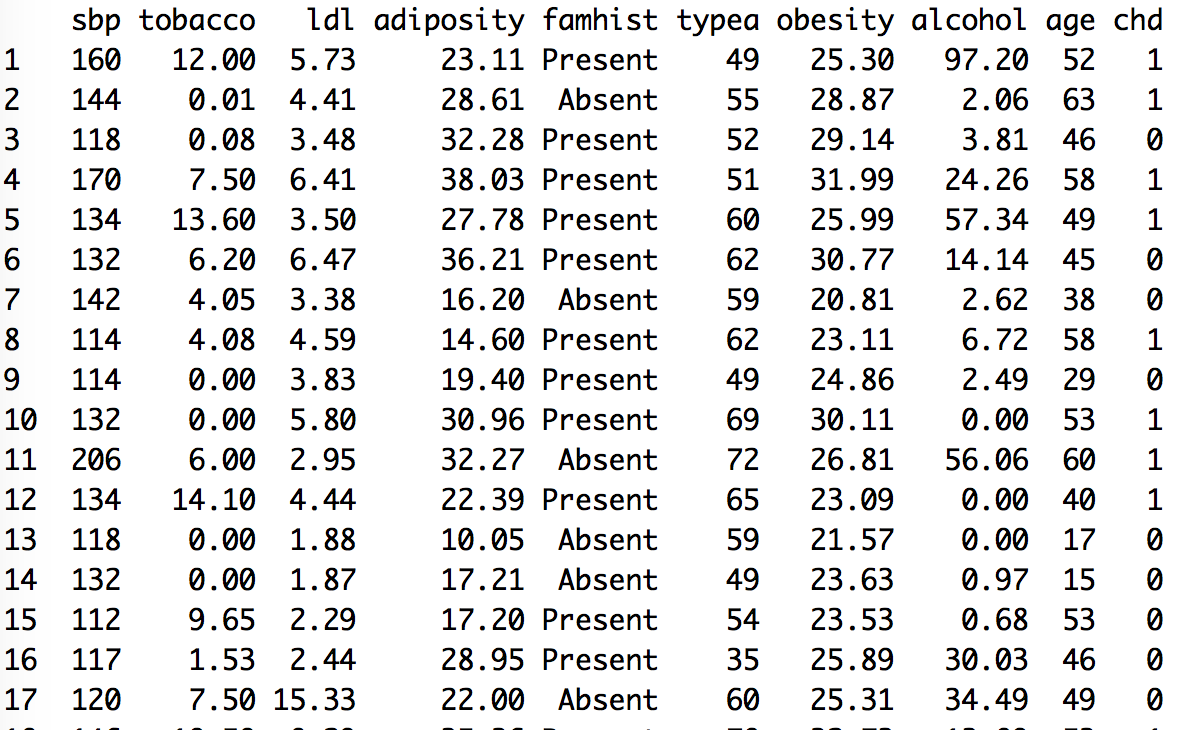
\includegraphics[width=4in]{SAheart_data}
      \caption{South African Heart Data from ESL}
    \end{figure}

    As you can see, some of the features are numerical and some categorical. You can
download this data from the book's website and have fun trying different
classifiers on  it.


  \subsection{Plotting and imagining a feature space $\R^d$ with binary labeled data}

  Try to imagine a training sample for binary classification in $\reals^d$,
  namely, points in $\reals^d$ that come with a label in $\left\{ 1,-1
  \right\}$ (say). 
  In the slides and handout, we can only plot examples in $\reals^2$, like the
  one below, but you
  should always try to imagine a higher-dimensional case.
  
  \begin{figure}[h!]
      \centering
      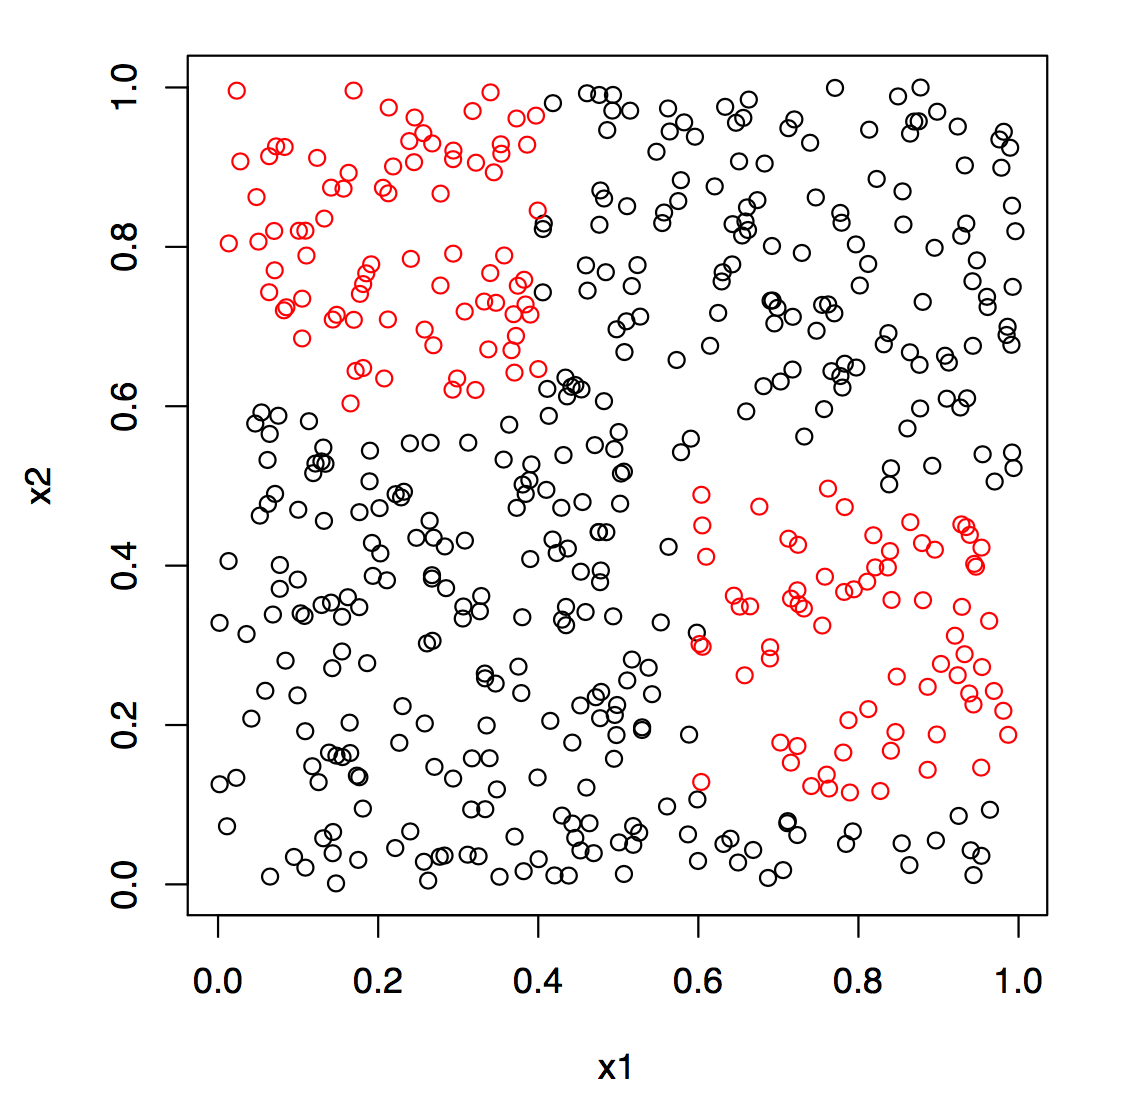
\includegraphics[width=4in]{tree1}
      \caption{Classification training sample in $\reals^2$}
    \end{figure}
 
   

  \subsection{What loss function should we use?}

  Recall from the linear regression lecture that we decided to measure
  performance using the {\bf square loss}. That was a reasonable choice for a
  regression problem. How shall we measure performance for {\bf classification?}

  \begin{itemize}
    \item The first idea is {\bf misclassification error}: simply count the
      samples in which the prediction and the true label did not agree. 
      Given a prediction (classification) rule $h:\X\to \left\{ \pm 1
      \right\}$, and a labeled sample $S=\left\{ (x_i,y_i \right\}_{i=1}^m$ (such as a
	training sample), the misclassification (or accuracy) 
	loss of $h$ on this sample will be 
	\[
	  L_S(h) := \sum_{i=1}^m \mathbf{1}_{y_i\neq h(x_i)} = 
	  |\left\{ i|y_i \neq h(x_i) \right\}|
	\]
      \item Can there be any problems or issues with the misclassification loss?
	After all, it just counts the number of times $h$ was  wrong - the number
	of times $h$ misclassified a sample. 
      \item The main problem is that - in practice - there are two kinds of
	errors the classifier can make, and making each kind of error can have
	very different implications, or costs. So just counting how many errors
	in total the classifier made may not be a useful performance measure. 
         \end{itemize}

    \subsection{Type-I and Type-II errors}
    \begin{itemize}
      \item {\bf Example: Credit decisions.}
       Suppose we are building a classifier that predicts whether a bank customer
	seeking a loan is
	credit-worthy and will return a loan if given one.  
	We choose the labels such that $-1$ means
	``not credit worthy, deny loan'' and $1$ means  ``credit worthy, approve
	loan''. What are the
	two kinds of {\bf errors} our classifier can make? 

      \item  Let the true label of a sample be $y_i$, and the classifier-predicted label
	 $\hat{y}_i$. If $y_i=-1$ and $\hat{y}_i=1$, the classifier predicted that a
	 non-credit-worthy customer will return the loan. If we act on this
	 prediction, and the customer defaults on the loan, the bank loses all
	 the loan sum. On the other hand, if $y_i=1$ and $\hat{y}_i=-1$, the
	 classifier predicted that a credit-worthy customer, which would have
	 paid the interest and returned the loan in full, is not credit-worthy
	 and should be denied the loan. If we act on this recommendation, the
	 bank loses the interest it would have earned on the loan. {\bf Which of
	 the two errors is more serious? Which of the two errors costs more to
       the bank?} If we could choose which error we should avoid ``at all
       costs'' and which error we can ``allow to happen'', what will we choose?

     \item {\bf Example: Drug safety.} Let's look at another example, an extreme
	 example to help illustrate this point. We are building a classifier
	 that predicts whether a certain drug is {\bf safe to use} for a
	 particular person, or {\bf unsafe} / deadly / dangerous to use.
	We choose the labels such that $-1$ means
	``unsafe drug, do not use'' and $1$ means  ``safe drug, ok to use''. 

	What are the two kinds of errors the classifier can make? 
	If $y_i=-1$ and $\hat{y}_i=1$, the classifier recommends to give a drug
	to a patient, which can actually kill them (say). 
	And if $y_i=1$ and $\hat{y}_i=-1$, the classifier recommends that the
	patient should avoid a
	drug, which is actually safe to use. 
	{\bf Which of the two errors is more serious?}
	If we could choose which error we should avoid ``at all
       costs'' and which error we can ``allow to happen'', what will we choose?

     \item So we see that, depending on the context of the
       classification problem, the two kinds of errors can have very different
       costs. The ``bad'' error, which we would like to avoid at all costs,
       is called Type-I error in the statistics literature. 
       The ``not-so-bad'' error is called Type-II error.

     \item In a classification problem we always choose one label in $\Y=\left\{
     \pm 1 \right\}$ and call it ``no effect'' or ``negative'' and the other
     ``effect'' or ``positive''. Suppose we called $-1$ ``negative'' and called
     $1$  ``positive''. 


Type-I and Type-II errors are defined as follows:

\begin{table}[h!]
          \centering
          \begin{tabular}{c|c|c}
            & $y_i=-1$ & $y_i=1$ \\ \hline
            $\hat{y}_i=-1$ &  $\cdot$ & \blue{Type-II error} \\ \hline
            $\hat{y}_i=1$ & \red{Type-I error} & $\cdot$ \\ \hline
          \end{tabular}
        \end{table}

      \item Choosing ``negative'' and ``positive'' defines which error is the
	Type-I error. For example, for the classification problem
	 ``Is the new drug safe to use?''\\
    We can assign the following meaning to the labels:\\
    $y=-1$: (negative) The new drug is safe\\
    $y=1$: (positive) The new drug is dangerous\\
           Then a Type-I error means: we decided not to offer a safe drug
\\~\\ 
But if we reverse the meaning to have  \\   
$y=-1$: (negative) The new drug is dangerous\\
$y=1$: (positive) The new drug is safe\\
  	\color{black}
        Then a Type-I error means: we decided to offer a dangerous drug. This is
	obviously the more serious of the two kinds of errors we can make.
  
      \item We always try to choose the ``negative'' and ``positive'' label such
	that the error we really want to avoid is the Type-I error - the error
	of taking a negative  sample and by mistake predicting it is 
	positive. 
  \item Exercise: For the classification problem of ``is this email spam or not'' how would
    you choose the labels? What are the two errors a spam detector can make?
    which one is the one we really want to avoid? So, which of the labels ``spam
    email'' and ``not spam, valid email'' would you label ``negative'' and which
    is ``positive''?
\end{itemize}

    \subsection{False Positive, False Negative and all that jazz}

    \begin{itemize}

  \item Here is important terminology you will hear with regards to
	classification errors.
    \item Assume the true label is $y=-1$ (no effect, negative).
      Then 
      \begin{itemize}
        \item  $\hat{y}=-1$ is {\bf true negative}
        \item  $\hat{y}=1$ is {\bf false positive}
      \end{itemize}
    \item Now assume the true label is $y=1$ (effect, positive).
      Then
      \begin{itemize}
        \item $\hat{y}=1$ is {\bf true positive}
        \item $\hat{y}=-1$ is {\bf false negative}
      \end{itemize}
    \item Note: false negative and false positives are the misclassification
      errors. False positive is what we called Type-I error, False negative is
      what we called Type-II error. True negative and true positve are the two
      cases where the classifier is {\bf correct}. It may take a little time to
      get used to this terminology. It's helpful to remember that something
      beginning with ``false'' is an error, and that the second word is the
      predicted label, not the true label. So that, for example, ``false
      positive'' is an {\bf error}, where we {\bf predicted} positive, so that the true
      label is actually {\bf negative}.

    \item Some more terminology:
    \begin{itemize}
     \item Denote $P$ number of positives, $N$ nuber of negatives
     \item Denote $TP$ and $FP$ number of true and false positives
\item Denote $TN$ and $FN$ number of true and false negatives
\item Then
  \begin{itemize}
    \item Error rate: $(FP+FN)/(P+N)$
    \item Accuracy $(TP+TN)/(P+N)$
    \item Precision: $TP/(TP+FP)$
    \item Recall (sensitivity, true positive rate): $TP/P$
    \item Specificity: $TN/N$
    \item False positive rate: $FP/N$
  \end{itemize}

   \end{itemize}
    \end{itemize}
 

    \subsection{Decision boundary}
    
    Let $h$ be a binary classification rule in $\reals^d$. (Suppose, for example, that
      we used a training sample to select $h$ from some hypothesis class $\Hc$. 
      We can feed any point $\VV{x}\in\reals^d$ into $h$ and get one of two
      classes. This means that $\reals^d$ is a disjoint union of two sets:
      \[
	\reals^d = \left\{ \VV{x}|h(\VV{x}=1 \right\} \biguplus \left\{
	    \VV{x}|h(\VV{x}=0 \right\}  
      \]
      (if the class labels are, say, $\Y= \left\{ 0,1 \right\}$).
      These sets can be very simple (two half-spaces) or very complicated.
      The boundary between these two sets is called the {\bf decision boundary}: 
      a test sample on one side of the boundary will be classified to one class
      by $h$, and a test sample on the other side of the boundary will be
      classified to the other class. 


      Figure \ref{b1} is a simple (in fact linear) decision boundary.
      \begin{figure}[h!]
      \centering
      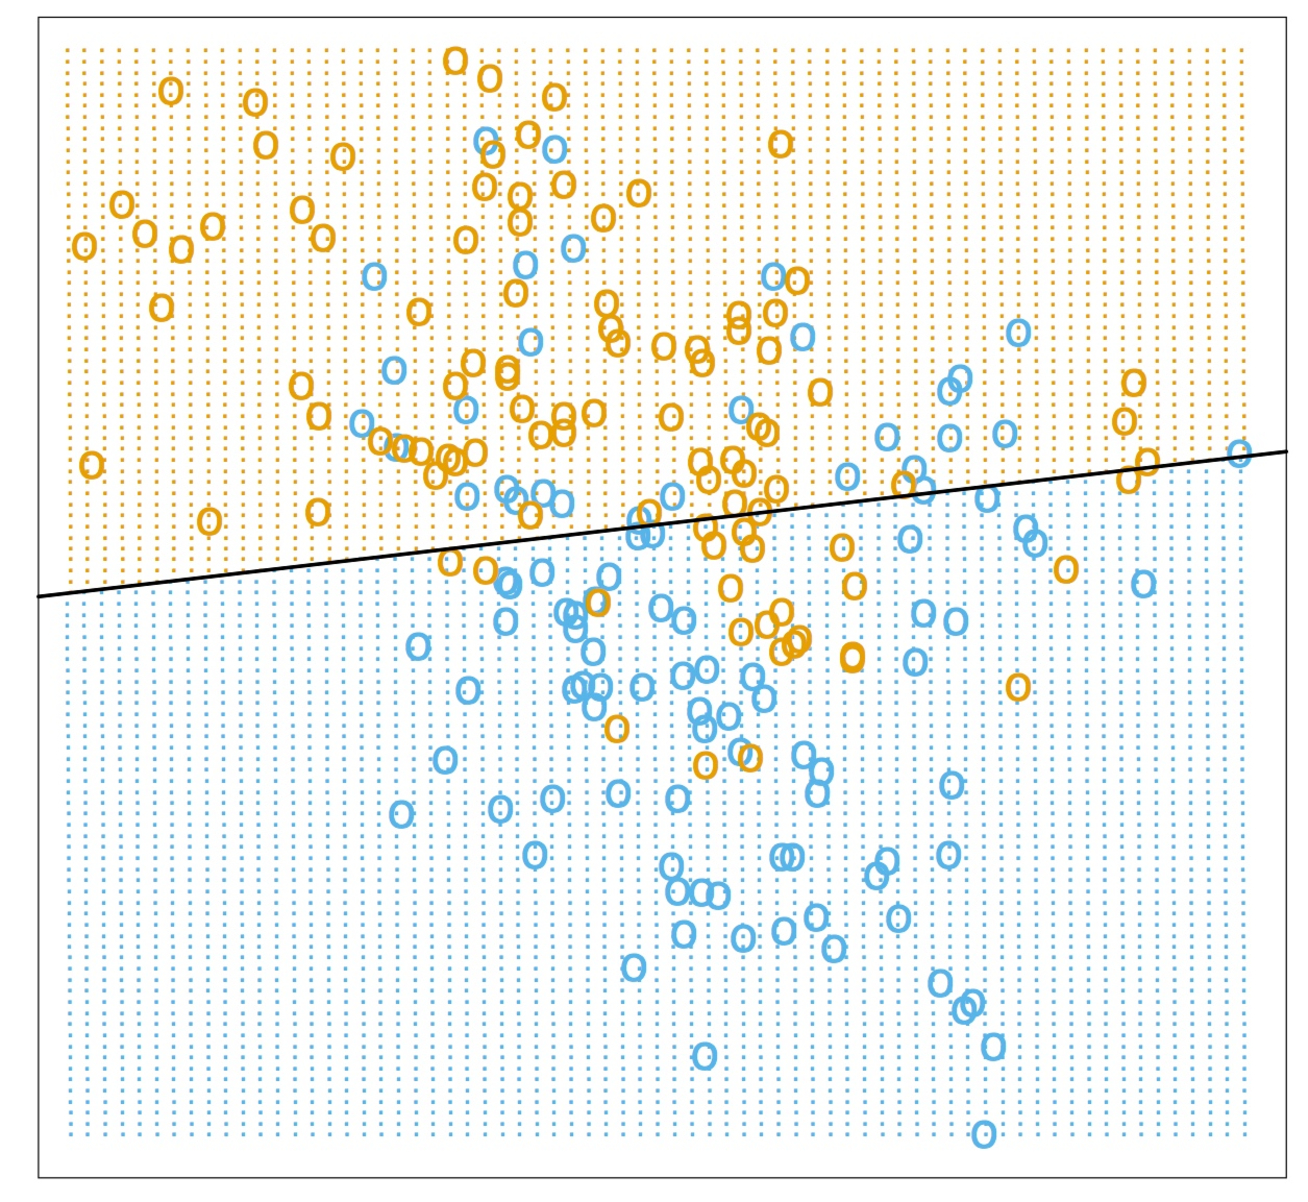
\includegraphics[width=3in]{b1.pdf}
      \caption{Decision boundary of a linear classifier (source: ESL)}
      \label{b1}
    \end{figure}

    Figure \ref{b2} is a more complicated decision boundary.

    \begin{figure}[h!]
      \centering
      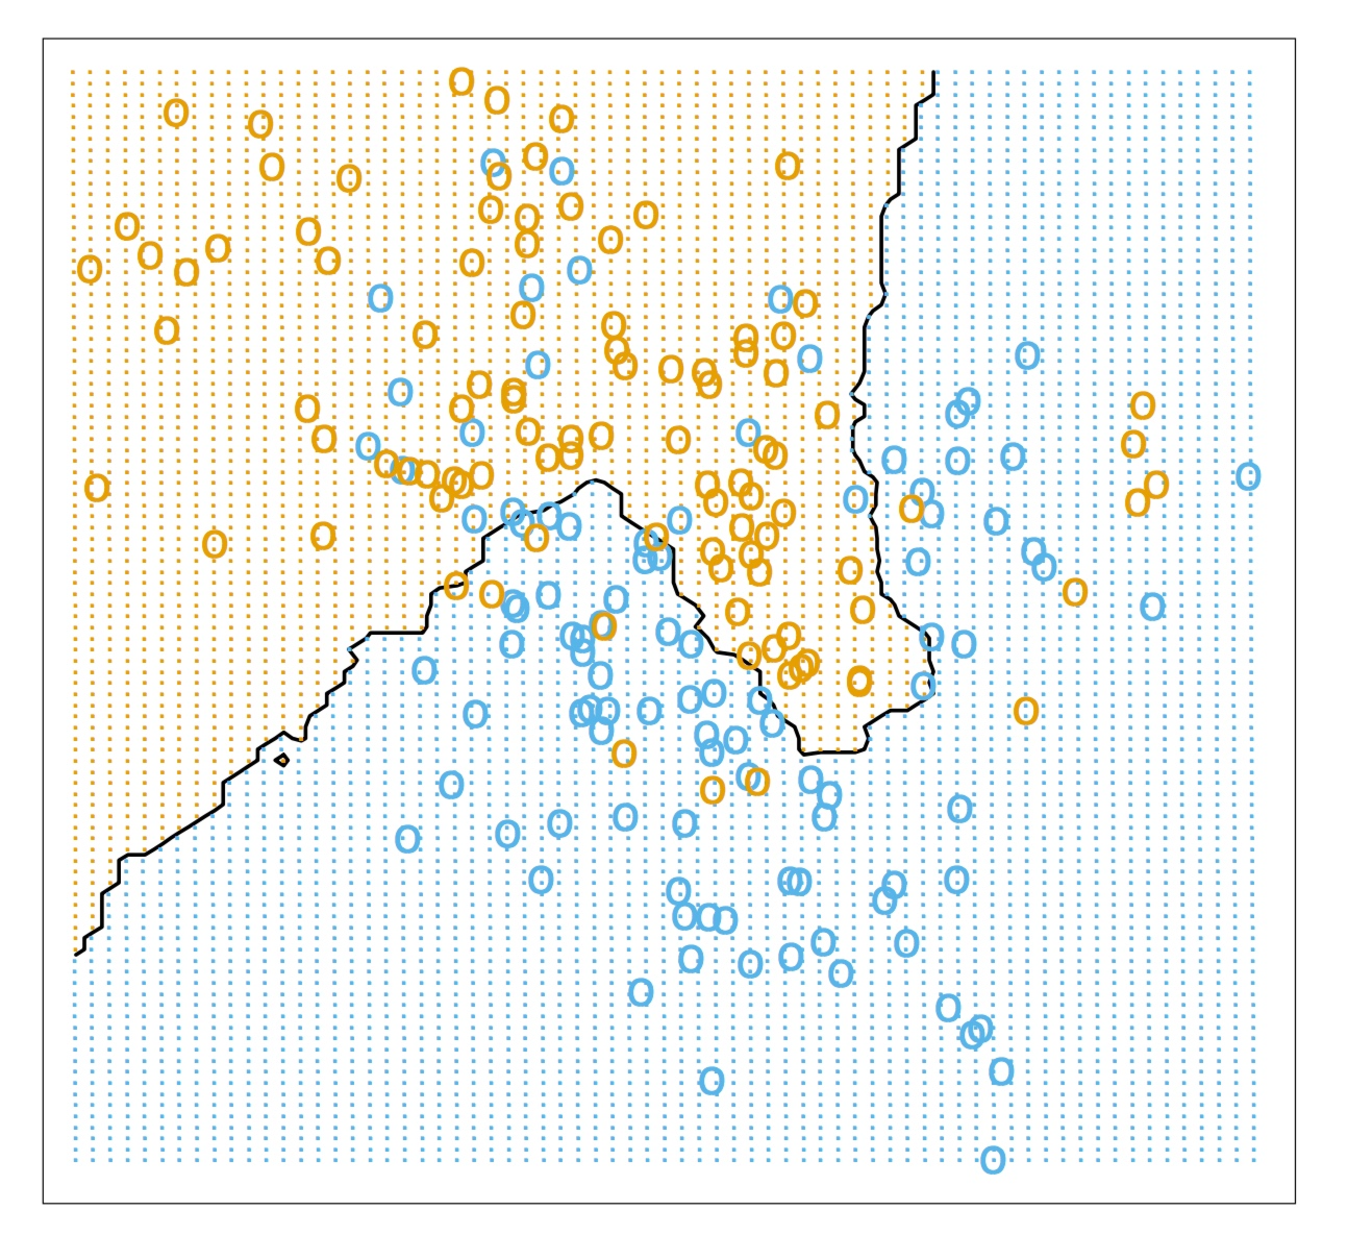
\includegraphics[width=3in]{b2.pdf}
      \caption{Decision boundary of a $k$-nearest-neighbor classifier (source:
	ESL}
	\label{b2}
    \end{figure}


      In learning a new classification method, it is useful to understand the
      {\bf shape} of the decision boundaries, to observe them in simulation, to
	plot them for real data, etc. This can help us develop intuition when we
	work we that classifier, and also get a qualitative assessment of the
	bias and the variance of that classifier. 
      
	\subsection{Our goal in this lecture}

	We will cover five very different classification algorithm. Our first
	goal is to be familiar with these methods, understand how they work, how
	and when to use them. Our second goal is to know {\bf how to read about
	a new classifier.} There are hundreds of methods our there, and as an
	expert, it's best to know which questions to ask when you approach a new
	learning algorithm, and what to key points you want to make sure you
	understand about it.

	Here is the list of questions we will ask about each method. Some of
	these questions will be explained as we go along.

\begin{itemize}
  \item What is the hypothesis class $\Hc$? How does the decision boundary look
    like?
  \item What is the learning principle for training model (choosing $h_S\in\Hc$
    based on training sample $S$)?
  \item How do we implement this principle computationally - how do we train the
    model and find $h_S\in\Hc$ in practice? What's the time complexity of this method?
    \item After training, how do we store trained model $h_S\in\Hc$? How much space
    is needed to store $h_S$?
  \item Given a trained model (namely, that we found $h_S\in\Hc$), how do we make
    predictions on new samples (namely, how do we compute $h_S(x)$ for a new
    sample $x\in\X$?) What is the time complexity of making a
    prediction for a single new sample?
  \item Is the learner interpretable?
  \item Does the learner provide estimated class probabilities?
  \item Is this a single model (a single hypothesis class $\Hc$), or actually a
    family of models (a family of hypothesis classes)? If a family, what are the
    parameters that choose the model from the family, and how do they affect the
    bias-variance tradeoff?
    \item When will we use this learning algorithm? What are its advantages and
      disadvantages?
\end{itemize}

%    \subsection{Multiclass classification}

\section{The Half-Space classifier}

Let's start with one of the simplest classifier imaginable. Our sample space is
$\reals^d$ and we have a training sample $S=\left\{ \left( \VV{x}_i,y_i \right)
\right\}_{i=1}^m$. It will be convenient to work with the class labels
$\Y=\left\{ +1,-1 \right\}$. 

Our hypothesis class $\Hc_{half}$ is the set of half-space classifiers in
$\reals^d$. These are functions of the form
\[
\VV{x} \mapsto \text{sign}\left( \innerr{\VV{x}}{\VV{w}} + b \right)\,.
\]
Each such function is completely determines by the vector $\VV{w}\in\reals^d$
and the scalar $b\in\reals$. (This should remind you of the linear regression
  hypothesis class\footnote{Indeed, While in linear regression we predicted a
  real-valued label with the class
  of linear functions (functions of the form $\VV{x} \mapsto
  \innerr{\VV{x}}{\VV{w}} + b$), now we predict a binary label with just a
level-set of a linear function.}.)

To see why the function $h_{\VV{w},b}(\VV{x}) = \text{sign}\left(
\innerr{\VV{x}}{\VV{w}} + b \right)$ is a half-space classifier, assume first
that $b=0$. Convince yourself that 
\[
  \reals^d = \left\{ \VV{x}\in\reals^d \,|\, \innerr{\VV{x}}{\VV{w}} > 0 \right\} \biguplus 
  \left\{ \VV{x}\in\reals^d \,|\, \innerr{\VV{x}}{\VV{w}} < 0 \right\} \biguplus 
  \left\{ \VV{x}\in\reals^d \,|\, \innerr{\VV{x}}{\VV{w}} = 0 \right\}
\]
and that these sets correspond to the open half space on one side of the
hyperplane $\VV{w}^\perp = \left\{ \VV{x}\in\reals^d \,|\, \innerr{\VV{x}}{\VV{w}} = 0
\right\}$, the open half space on the other side of that hyperplane, and points
on the hyperplane itself. So each vector $\VV{w}\in\reals^d$ defines a
hyperplane $\VV{w}^\perp$ and divides $\reals^d$ into two half-spaces. 
\\~\\
\begin{figure}[h!]
  \centering
  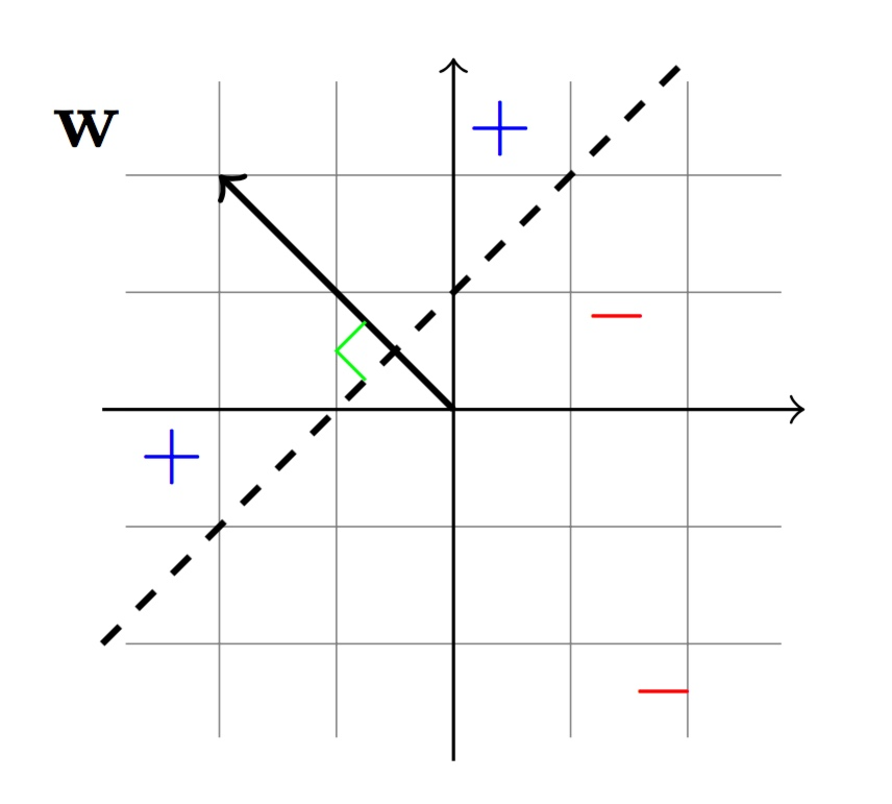
\includegraphics[width=3in]{half.pdf}
  \caption{Half-space defined by a vector. Source: UML}
\end{figure}

The case $b=0$ is called the {\bf homogeneous} case, as the hyperplane
$\VV{w}^\perp$ runs through the origin of $\reals^d$. When $b\neq 0$,  the
hyperplane does not run through the origin.

\subsection{Assumption - training sample is linearly separable}

Let's start with the
unreasonable assumption that the training samples are {\bf linearly separable},
in the sense that there exists a hyperplane for which all training samples
labeled $1$ are on one side and all training samples labeled $-1$ are on the
other side. 

Mathematically, this means that we assume that, for our training sample $S$, 
there exist a vector $\VV{w}\in\reals^d$ and a scalar $b\in\reals$ such that 
$y_i \cdot \text{sign}\left( \innerr{\VV{x}}{\VV{w}} + b \right) =1$ for all $i$, or
equivalently
\[
y_i \cdot \left( \innerr{\VV{x}}{\VV{w}} + b \right) > 0\qquad 
i=1,\ldots,m
\]
since the inner product will be negative for samples with $y_i<0$ and positive
for samples with $y_i>0$. (If we chose $\VV{w}$ pointing at the ``wrong
  direction'', we will have $y_i \cdot \text{sign}\left( \innerr{\VV{x}}{\VV{w}}
+ b \right) <0$. In this case we just change $\VV{w}$ to $-\VV{w}$.)

{\bf For simplicity, let's work with
the homogeneous case $b=0$.} (We can always shift the entire training sample by a
  fixed vector if needed, to make sure that the separating hyperplane runs
through the origin.)
\\~\\
So our hypothesis class is 
\[
  \Hc_{half} = \left\{  h_\VV{w}: \VV{x} \mapsto \text{sign}\left( \innerr{\VV{x}}{\VV{w}}  \right)
\,\big|\, \VV{w}\in \reals^d \right\}
\]
and, just like in linear regression, training the model reduces to finding
vector $\VV{w}\in\reals^d$. Note that our assumption that the training sample is
linearly separable is known as the {\bf realizability assumption} - namely, {\bf that
the labels are generating by a function in our hypothesis class.}

\subsection{Learning using ERM}

Now that we have our hypothesis class, how do we train the model - namely, how
do we choose $h\in\Hc_{half}$ given a training set?

Observe that, for a hypothesis $  h_\VV{w} \in \Hc_{half}$,  the misclassified
training 
samples are exactly those samples with 
$y_i \cdot \text{sign}\left( \innerr{\VV{x}}{\VV{w}}\right) = -1$ or equivalently 
$y_i \cdot \innerr{\VV{x}}{\VV{w}}  <0$

The loss of $ h_\VV{w}$ on the training sample $S$ is therefore
\[
  L_S( h_\VV{w}) = \sum_{i=1}^m \mathbf{1}_{y_i \cdot 
  \innerr{\VV{x}}{\VV{w}} <0}
\]

Since the training
sample is linearly separable by assumption, clearly it makes sense to choose $h\in\Hc_{half}$ 
that perfectly separates the training sample. Such $h\in\Hc_{half}$ will have
zero training loss, $ L_S( h_\VV{w}) =0$.
In other words, any separating hyperplane $\VV{w}^\perp$ is going
to correspond to an hypothesis $h_\VV{w}$ that minimizes the empirical risk 
$  L_S( h_\VV{w})$. (By assumption, the minimal value will be $0$).
So we decide that the learning principle will again be {\bf
empirical risk minimization -  the same principle we used for developing
linear regression.} 

\subsection{Computationally implementing ERM for halfspace classifiers}

The question is now if there is a computationally efficient way to find
\[  \text{argmin}_{\VV{w}\in\reals^d} L_S(h_\VV{w})\,.\]

By assumption there exists a vector $\VV{w_0}\in\reals^d$ such that
\[
y_i \cdot \innerr{\VV{x}}{\VV{w_0}}  > 0\qquad 
i=1,\ldots,m
\]

First observe that this implies that there also exists a (different) vector
 $\VV{w_1}\in\reals^d$ such that
 \[
y_i \cdot \innerr{\VV{x}}{\VV{w_1}}  \geq 1 \qquad 
i=1,\ldots,m
\]
To see why this is true, just normalize $\VV{w_0}$ by the smallest product,
namely, define 
\[
  \VV{w_1} := \frac{1}{ \min_i \{y_i \cdot 
  \innerr{\VV{x}}{\VV{w_0}} \}  }\cdot \VV{w_0}\,.
\]

So it's enough to look for a vector $\VV{w}$ that satisfy
 $
y_i \cdot \text{sign}\left( \innerr{\VV{x}}{\VV{w}} \right) \geq 1 \qquad 
i=1,\ldots,m
$

We are looking for a vector that  satisfies $m$ linear constrains. Of course we
know how to do this - linear programming.

\subsection{Commercial break: Convex optimization}

Before we continue with half-spaces, let us break and briefly introduce convex
optimization, since we will start using convex optimization tools and concepts.

\begin{itemize}
  \item {\bf An optimization problem} over $\reals^d$ has the general form
    \begin{eqnarray*}
      \text{minimize} & f_0(\VV{x}) & \\
      \text{subject to} & f_i(\VV{x}) \leq b_i, & \qquad i=1\ldots n
    \end{eqnarray*}
    where $\VV{x}$ is the {\bf optimization variable}, $f_0:\reals^d\to\reals$ is
    the {\bf objective function},  and  $f_i:\reals^d\to\reals$ ($i=1,\ldots,m$) are
    the {\bf constraint functions}. It is implicitly implied that 
    the optimization happens over $dom(f_0)\subset
    \reals^d$, the domain of $f_0$.
  \item {\bf A convex function} is
    function $f:\reals^d\to\reals$ such that $dom(f)$ is a
    convex set in $\reals^d$, and 
    \[
      f(\alpha \VV{x} + \beta \VV{z}) \leq  \alpha f(\VV{x}) + \beta f(\VV{z})
    \]
    for all $\alpha,\beta\in\reals$ and all $\VV{x},\VV{z}\in dom(f)$.

  \item {\bf A convex  optimization problem} is an optimization problem as above
    in which $f_0,f_1,\ldots, f_n$ are all convex functions.
  \item {\bf A linear programming problem (or a linear program)} 
    is a special case of a convex optimization problem, in which 
    $f_0,f_1,\ldots, f_n$ are all {\bf linear} functions.

\end{itemize}


In general, optimization problems are hard to solve computationally. We take
special interest in {\bf convex optimization} problems since there have a unique
solution, and that solution can be found in  computationally tractable ways. A
great deal is known about {\bf convex optimization algorithms}, which are
iterative numerical algorithms that converge to the solution of a convex
optimization problem. There are general solvers, which will solve a convex
problem in the general form above, and there are specialized solvers for specific
types, or families, of convex optimization problems. A specialized solver is
typically preferred, as it leverages some particular structure of the problem to
solve it more efficiently, using less space, etc. One example for specialized
solvers you've seen in Algorithms course are specialized solvers for linear
programs.
\\~\\
Why is convex optimization interesting for machine learning? In supervised
learning, we would like to choose a hypothesis $h\in\Hc$ from our selected
hypothesis class, based on some learning principle (such as ERM). Many learning
principles are formulated as optimization problems, namely, the $h$ our learning
algorithm chooses is
given as the minimizer of some quantity (such as empirical risk). So
implementation of the
learning algorithm needs to solve an optimization problem. 

Sometimes, our hypothesis class is equivalent to a Euclidean space (for example, in
  linear regression we saw that linear functions are determined by the weight
  vector and an intercept, so the hypothesis class of linear functions was equivalent to 
the Euclidean space $\reals^{d+1}$, and we've just seen the same happens for
the hypothesis class of half-space classifiers). When this happens, our learning
principle reduces to solving an optimization problem, namely, the hypothesis we
choose $h\in\Hc$ is found as a minimum over $\reals^d$ or a subset of $\reals^d$
of some objective function, usually a loss function. When this objective is convex,
we can use convex optimization algorithms to implement our learning algorithm
 efficiently. 

(We will have a future lecture dedicated to theory and
algorithms of convex
optimization.)

\subsection{Solving ERM for half-space by linear programming}

Back to the half-space classifier. 
We saw that a hyperplane $\VV{w}^\perp$ minimizing ERM is a solution to the
following linear program:
 \begin{eqnarray*}
      & \text{minimize}   & 0 \\
     & \text{subject to} &  y_i \cdot  \innerr{\VV{x}_i}{\VV{w}}
       \geq 1  \qquad 
i=1,\ldots,m
    \end{eqnarray*}

    Such an optimization problem (with trivial objective) is called a {\bf
    feasibility} problem - we're just looking for any vector which satisfies the
    constrains. 
\\~\\
So, one way to implement ERM for the half-space classifier is using linear
programming. There is another famous way, known as the {\bf Perceptron} algorithm.
This is an iterative algorithm with a guaranteed rate of convergence to a
solution. You'll see this algorithm in the recitation.


\subsection{What about a training sample that's not linearly separable?}

When the sample training is not linearly separable, the optimization problem
above has no solution. We can still try to implement the ERM principle (find a
hyperplane with minimal number of misclassification errors) however
unfortunately in this case 
the minimization problem 
\[  \text{argmin}_{\VV{w}\in\reals^d} L_S(h_\VV{w})\,.\]
is known to be  computationally hard. 




\subsection{Summary}
\begin{itemize}
  \item Hypothesis class $\Hc$: Half-spaces
  \item Learning principle for training model (choosing $f\in\Hc$): Separating
    hyperplane chosen with Empirical Risk Minimization
    (ERM) for misclassification loss
  \item Computational implementation of learning principle: Linear programming, Perceptron
  \item How to store trained model: store the vector $\VV{w}$ perpendicular to
    the hyperplane defining the half-space  
  \item When to use: As a simple baseline. Otherwise never.
\end{itemize}


See if you can fill in these yourself:
\begin{itemize}
  \item How to make predictions on new samples?
  \item Time complexity for training, and for predicting on a new sample?

\end{itemize}

\section{Support Vector Machines}

We encountered two problems with the half-space classifier. 
\begin{itemize}
  \item 
    Even if the training sample is linearly separable, the half-space separating
    is not unique. Which one should we choose? (see figure - which of the
    hyperplanes should we choose?)

    \begin{figure}[h!]
      \centering
      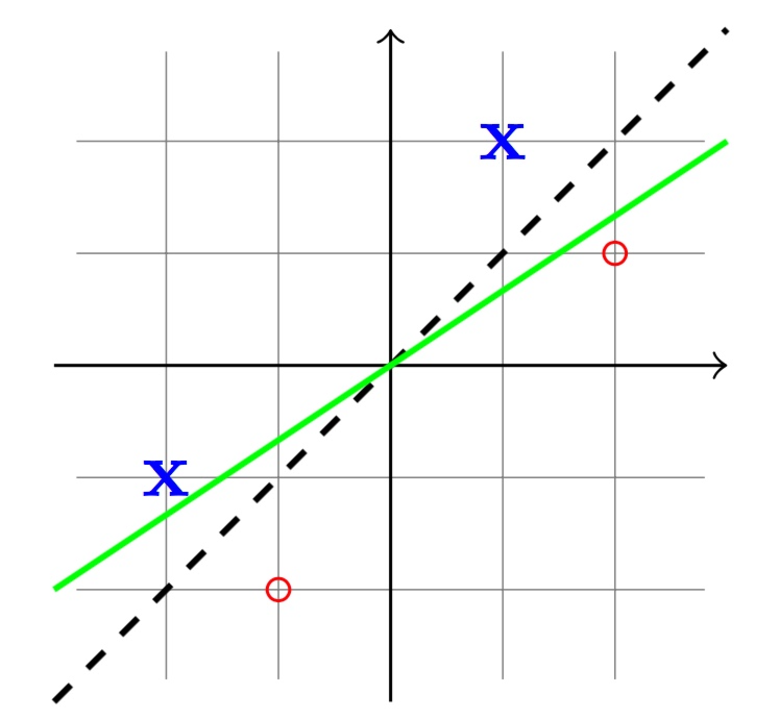
\includegraphics[width=3in]{nonuniq.pdf}
      \caption{Which separating hyperplane should we choose? Source: UML}
    \end{figure}


  \item A much more severe problem is that we chose to work with the ERM
    principle to select the hypothesis $h$, but when the training sample is not
    linearly separable, implementing ERM is computationally hard. So the
    half-space classifier is not very useful in practice. 
    
\end{itemize}

We'll now continue with the same hypothesis class if half-spaces. We won't
assume that they are defined by hyperplanes that go through the origin. So our
hypothesis class is now
\[
  \Hc_{SVM} = \left\{  h_\VV{w}: \VV{x} \mapsto \text{sign}\left(
  \innerr{\VV{x}}{\VV{w}}  +b \right)
\,\big|\, \VV{w}\in \reals^d, b\in \reals \right\}
\]


But we won't use the ERM principle. We will 
introduce a totally different learning principle, one which solves both problems
above. It gives us a unique hyperplane, and it can be implemented
computationally - efficiently - even when the training sample is not linearly
separable. You'll cover SVM again in the recitation, so this will part of the lecture
will be relatively fast and a little less detailed. 



\subsection{A new learning principle: Maximum Margin}


For a hyperplane $(\VV{w},b)$ (defined by the vector $\VV{w}\in\reals^d$ and a
scalar $b$) and
point $\VV{x}\in\reals^d$, define the {\bf distance} between $(\VV{w},b)$ and
$\VV{x}$ by 
\[
  D( (\VV{w},b) , \VV{x}) := \min_{\VV{v}:\innerr{\VV{v}}{\VV{w}}  +b=0  } \norm{\VV{x}-\VV{v}}
\]
namely the Euclidean distance between $\VV{x}$ and the closest point on the
hyperplane $(\VV{w},b)$.
\\~\\
Now let's define the {\bf margin} of  a hyperplane, with respect to a training
sample $S=\left\{ \left( \VV{x}_i,y_i \right) \right\}$. The margin $M\left(
   (\VV{w},b) , S
 \right)$ is simply the smallest distance between the hyperplane and any sample
 point $\VV{x}_i$:
\[
  M( (\VV{w},b) , S) := \min_{1\leq i\leq m} D( (\VV{w},b) , \VV{x}_i)\,.  
\]
Obviously, a hyperplane with a large margin is preferred - since, if it
separates the training samples, the larger the margin, the better the
separation.
\\~\\
Our new learning principle is: 
 We will choose $h_{\VV{w},b} \in
 \Hc_{SVM}$ that has the {\bf largest margin} with respect to our training sample $S$. 
\\~\\
The vectors closest to the hyperplane determine the margin. They are called {\bf
support vectors}, hence this learner's name. (Calling it a support vector {\bf
machine} has no justified reason, but is just cool.)

 \subsection{Hard SVM}
 Let's start with the {\bf realizable case}, namely make the same assumption we
 had for the half-plane classifier - that the training sample is linearly
 separable. (We'll remove this soon.)
 To implement our learning principle of maximal margin, we need to search, among
 all the hyperplane separating $S$, for the hyperplane with maximum margin. 
 Namely, the hypothesis $h_{\VV{w},b} \in
 \Hc_{SVM}$ our learner will choose is the solution to the following
 optimization problem
  \begin{eqnarray*}
      & \text{maximize}   &  M( (\VV{w},b) , S) \\
     & \text{subject to} &  y_i \cdot \left( \innerr{\VV{x}_i}{\VV{w}}
      +b \right) \geq 1  \qquad 
i=1,\ldots,m
    \end{eqnarray*}
    The optimization variables are $\VV{w}\in\reals^d,b\in\reals$. (Compare this
      to the linear program above for half-spaces: we kept the same constrains,
      which ensure that the hyperplane chosen will separate the training sample,
    but, instead of a trivial objective, we have the margin!) We don't worry
    about ``maximize'' instead of ``minimize'' as we can just multiply the
    objective by $-1$. 
\\~\\
Is this a convex optimization problem? We hope so, since if yes, it is
computationally tractable. 
\\~\\
{\bf Exercise.} If $\norm{\VV{w}}=1$ then $ D( (\VV{w},b) = 
  |\innerr{\VV{x}}{\VV{w}}+b|$.  (The solution is in ``Understanding Machine
  Learning'' claim 15.1).
\\~\\
We don't mind describing the hyperplane using a unit vector - it really doesn't
matter. So our optimization problem is equivalent to:
\begin{eqnarray*}
  & \text{maximize}   &  \min_{1\leq i\leq m} |\innerr{\VV{x}_i}{\VV{w}}+b| \\
     & \text{subject to} &  y_i \cdot \left( \innerr{\VV{x}_i}{\VV{w}}
      +b \right) \geq 1  \qquad 
i=1,\ldots,m
    \end{eqnarray*}
    \\~\\ Well, is this convex? In the recitation you'll see that this problem
    is equivalent to the following optimization problem:
    \begin{eqnarray*}
      & \text{minimize}   &  \norm {\VV{w}}^2 \\
     & \text{subject to} &  y_i \cdot \left( \innerr{\VV{x}_i}{\VV{w}}
      +b \right) \geq 1  \qquad 
i=1,\ldots,m
    \end{eqnarray*}
    \\~\\ So, good news - you can see that in this latest optimization problem,
    the objective is convex (the norm function is convex by triangle inequality)
    and, as before, the constrains are linear. 
    A convex optimization problem in which the objective is a quadratic form of
    the optimization variable, and the constrains are linear functions, is
    called {\bf a Quadratic Program} (QP). This is one of those special families
    of convex optimization problems that we mentioned. There are specialized
    solvers for Quadratic Programs that are much more efficient that general
    convex solvers. 
  \\~\\
  This version of SVM is called {\bf Hard SVM} (for ``hard margin'') and is
  only suitable for a separable training sample - indeed, if the training sample
  is not separable, the optimization problem above has no solutions as for any
candidate $\VV{w},b)$, at least
  one of he 
  constrains 
  \[
    y_i \cdot \left( \innerr{\VV{x}_i}{\VV{w}}
      +b \right) \geq 1  
  \]
  cannot be satisfied. 

  \subsection{Soft SVM}

  This last sentence gives us an idea. We can't really expect that the training
  sample will be linearly separable, meaning that we can't expect {\bf all} the
  constrains
   \[
    y_i \cdot \left( \innerr{\VV{x}_i}{\VV{w}}
      +b \right) \geq 1  
  \]
  to be satisfied simultaneously. So we would like to allow this constrain to be
  violated - for as few training samples as possible, of course. Recall that if
  $ y_i \cdot \left( \innerr{\VV{x}_i}{\VV{w}}
  +b \right) <0$, this means that the sample $\VV{x}_i$ is on the ``wrong side''
  of the hyperplane. Similarly, convince yourself that if there exists some
  $\xi_i>0$ such that 
  \[
  y_i \cdot \left( \innerr{\VV{x}_i}{\VV{w}}
+b \right) \geq 1-\xi_i  \]
this means that the sample $\VV{x}_i$ is  on the wrong side of the {\bf margin}
by a proportional amount of $\xi$ (try to understand mathematically the exact meaning of this
sentence.)
\\~\\ So in order to allow training samples to violate the constrains ``a
little'', and end up on the wrong side of the margin, we change the Hard-SVM
optimization problem to:
\begin{eqnarray*}
      & \text{minimize}   &  \norm {\VV{w}}^2 \\
      & \text{subject to} & \begin{cases} y_i \cdot \left( \innerr{\VV{x}_i}{\VV{w}}
     +b \right) \geq 1-\xi_i  \,\,\text{and}\,\, \xi_i\geq 0 \qquad 
i=1,\ldots,m & \\
 \frac{1}{m}\sum_{i=1}^m \xi \leq C &
 \end{cases}
    \end{eqnarray*}
    where $C>0$ is a constant that we specify. The variables $\xi_1,\xi_m$ are
    new auxiliary variables that we introduced. This is still a Quadratic
    Program.
    \\~\\
    The larger the constant $C$ we choose, the more violations of the margin we
    allow. One the one hand, we want to allow ``noisy'' samples to violate the
    margin, so that the hyperplane will ignore them; on the other hand, 
    if we allow to many violations, we lose touch with the training sample and
    its structure. This is exactly the bias-variance tradeoff: basically, the
    larger $C$, the more freedom the learner has to ``chase after the training
    sample''. 
\\~\\
Another possibility for allowing violations is as follows:
\begin{eqnarray*}
      & \text{minimize}   &  \lambda \norm {\VV{w}}^2 + \frac{1}{m}\sum_{i=1}^m
      \xi_i \\
      & \text{subject to} & y_i \cdot \left( \innerr{\VV{x}_i}{\VV{w}}
     +b \right) \geq 1-\xi_i  \,\,\text{and}\,\, \xi_i\geq 0 
    \end{eqnarray*}
    Here, instead of specifying the constant $C$, we specify a constant
    $\lambda$ that is included in the optimization problem's objective. The
    larger $\lambda$, the less sensitive the solution will be to the term $\frac{1}{m}\sum_{i=1}^m
    \xi_i$, and will allow more violations. 
    The smaller $\lambda$, the more sensitive, and will allow less violations.
    If we choose to work with this optimization problem to choose $h$, the
    constant $\lambda$ also moves us along different members of a family of
    learners, each with a different bias-variance tradeoff. $\lambda$ is known
    as a {\bf regularization parameter} - we will have a lecture about
    regularization later in the course, and will understand more about learners
    based on optimization problems that contain a regularization term.


    \subsection{A family of learners}

    In Soft SVM, we encounter something new and important: the soft SVM
    algorithm requires a parameter $C$ or $\lambda$. The hypothesis produced by
    the learner - for a given training sample - depends heavily on the
    parameter. So in fact, Soft-SVM is not a single learning algorithm, but a
    family of learning algorithms. Changing $C$ 

    \subsection{When is SVM useful?}

    Since the hypothesis class of SVM is half-spaces, it is generally a
    classifier with high bias and low variance. SVM is useful in high
    dimensions, when the dimension $d$ is large. In the recitation, you will see
    a method to ``lift'' a sample into a space with higher dimensions, where it
    can become linearly separable or almost linearly separable - and then SVM
    can be useful.




\subsection{Summary - Soft SVM}
\begin{itemize}
     \item Hypothesis class $\Hc$: Half-spaces
     \item Learning principle for training model (choosing $f\in\Hc$): Linear separator with Maximum Margin
    \item Computational implementation of learning principle: Quadratic Program
  \item How to make predictions on new samples:       
  \item Interpretable: No
    \item Estimates class probabilities: No
  \item Family of models: Yes, indexed by the regularization parameter
    $\lambda\in[0,\infty)$.
     \item Time complexity for training, and for predicting on a new sample:
  \item How to store trained model: store the vector $\VV{w}$ perpendicular to
    the separating half-space  
  \item When to use: (i) As a simple baseline (ii) after embedding data in
    high-dimensional space (kernelization) - see next recitation. 
\end{itemize}


\section{Logistic Regression}
\subsection{A probabilistic model for noisy labels}
\begin{itemize}
  \item One way to think about linear regression with Gaussian errors: 
    Assumed $y=f(\VV{x})$ for $f$ a linear function in the sample vector $\VV{x}$.
    With noise, each label $y_i$ is drawn from a random variable of the form
    $y_i = \innerr{\VV{x_i}}{\VV{w}}  + z_i$ with $z_i \sim \Nc(0,\sigma^2)$.
    Equivalently
    $y_i \sim \mathcal{N}( \innerr{\VV{x_i}}{\VV{w}} , \sigma^2)$. 
    We want to learn the vector $\VV{w}$ (or equivalently, the linear function
      $\VV{x}\mapsto f(\VV{x})$. 
      In other words, we assumed that each sample $(\VV{x},y)$ is such that
      the {\bf expected value} of the label $y$ is
      linear in $\VV{x}$. 
    \item For classification on $\X=\reals^d$, we have samples $(\VV{x},y)$ with
      $\VV{x}\in\reals^d$ and $y\in\left\{ \pm 1 \right\}$. When discussing
      logistic regression it is convenient to use labels $\{0,1\}$ instead. 
      Let's assume a probabilistic model similar to that of linear regression:
      it's natural to use {\bf Bernoulli} random variables. Can we want to assume 
      $y_i \sim Ber(p_i)$, for some $p_i\in[0,1]$ that's related somehow to
      $\VV{x}_i$. This models noise: each sample is a result of some ``inner''
      tendency to be $0$ or $1$, which we called $p_i$, but then a coin is
      flipped to determine $y_i$. It could be that $p_i$ is very small and by
      chance we drew $y_i=1$, for example - but that would be rare. So this is a
      good model for labels in $\{0,1\}$ that come with noise.  
    \item How shall we connect $p_i$ to $\VV{x}_i$? We can't assume a linear
      function $\innerr{\VV{x_i}}{\VV{w}}$ for some $\VV{w}\in \reals^{d+1}$, as in linear regression, since $p_i$ is
      restricted to $[0,1]$. So it would be natural to choose a {\bf link}
      function $\phi:\reals\to[0,1]$ that is monotone increasing, and maps
      $(-\infty,\infty)$ bijectively to $(0,1)$,  and assume
      that $p_i = \phi (\innerr{\VV{x_i}}{\VV{w}} ) $ for some
      $\VV{w}\in\reals^{d+1}$.  
    \item 	Why is $\VV{w}\in\reals^{d+1}$ and not  $\VV{w}\in\reals^{d}$?
	just like in linear regression, we need an {\bf intercept}. So we pad
	the sample vectors $\VV{w}$ with a $1$ in the $0$-th entry, so that 
	$\innerr{\VV{x_i}}{\VV{w}} = \sum_{j=0}^d x_j w_j = w_0 +\sum_{j=1}^d x_j
	w_j$ where $\VV{x}=(1,x_1,\ldots,x_d)$ and $\VV{w}=(w_0,w_1,\ldots,w_d)$.
    \item So our model is that labels are independent of each other, and that
      there exists a vector $\VV{w}$ such that  $y_i \sim Ber(\phi
      (\innerr{\VV{x_i}}{\VV{w}} ))$.
      This hypothesis class is indexed by the vector $\VV{w}\in\reals^{d+1}$ - and just like
      linear regression, learning comes down to finding $\VV{w}$. 
    \item What function shall we use for $\phi$? There are a few well known choices in the
      literature. Honestly it doesn't matter all that much, as long as the
      function $\phi:\reals\to[0,1]$ that is monotone increasing, and maps
      $(-\infty,\infty)$ bijectively to $(0,1)$ (so that it's invertible). 
      We would like $\phi$ to be smooth, so that we can use derivatives in
      any optimization that will be needed to train the model and choose $\VV{w}$
      based on the training sample. 
    \item The $\phi$ we will use is the famous {\bf logistic function}
      \[\pi(x) = \frac{e^x}{1+e^x}\,.\] (verify that it is smooth, indeed
	analytic,  monotone increasing, and maps
      $(-\infty,\infty)$ bijectively to $(0,1)$). 
  \end{itemize}
  \subsection{The hypothesis class}
  \begin{itemize}
    \item So our hypothesis class is simply 
      \[
	\Hc_{logistic}^d= \left\{ \VV{x} \mapsto \pi(\innerr{\VV{x}}{\VV{w}} ) \right\}\,.
      \]
      But wait, something is not right.  We are in a classification lecture, where
      $\Y=\left\{ 0,1 \right\}$, but this hypothesis class contains functions 
      $\reals^{d+1} \to [0,1]$, not $\reals^{d+1} \to \left\{ 0,1 \right\}$. 
      Since $\left\{ 0,1 \right\}\subset [0,1]$, we can use
      our classification training sample to choose a function in
      $\Hc_{logistic}^d$. So we'll
      be able to train the model. But how will we 
      predict on a new sample? If our learner chose some $h\in\Hc_{logistic}^d$, and
      equivalently some $\VV{w}\in \reals^{d+1}$, how do we predict a label
      $\left\{ 0,1 \right\}$ for some sample $\VV{x}$? The value $h(\VV{x})$ is in
      $[0,1]$ and may be, for example, $0.7$. And we need a classifier, so need
      a value in $\left\{ 0,1 \right\}$, not in $[0,1]$.
      The answer is that we think about $h(\VV{x})$ as an estimate of the
      probability that the label corresponding to $\VV{x}$  is $1$. If
      $h(\VV{x})=0.1$, the label is likely $0$. If $h(\VV{x})=0.9$, the label is
      likely $1$. We will need to choose a {\bf cutoff} $\alpha$ and our class
      prediction will be 
      \[\hat{y} := \begin{cases} 1 & h(\VV{x})>\alpha \\ 0 &
      h(\VV{x}) \leq \alpha \end{cases}\,.\]
      {\bf More on how to choose the cutoff $\alpha$ - 
      soon. This is an important subject.}
      \end{itemize}
  \subsection{The learning principle: maximum likelihood}
  \begin{itemize}
    \item Back to logistic regression. So we have our hypothesis class 
      $\Hc_{logistic}^d$. What learning principle shall we use- how will we
      choose the function $h\in \Hc_{logistic}^d$, and, equivalently, the vector 
      $\VV{w}\in\reals^{d+1}$, from a training sample 
      $S=\left\{ (\VV{x}_i,y_i \right\}_{i=1}^m$?
      We will use the {\bf maximum likelihood principle} (seen in the
      linear regression lecture).
    \item Assuming that $y_i \sim Ber(\pi
      (\innerr{\VV{x_i}}{\VV{w}} ))$ where $\pi$ is the logistic function, and
      assuming the labels $y_i$ are all independent, we can write the {\bf joint
      density} of the labels vector $\VV{y}=(y_1,\ldots,y_m)\in\left\{ 0,1
      \right\}^m$. Let $Y=(Y_1,\ldots,Y_m)$ be a random vector taking values in
      $\left\{ 0,1 \right\}^m$ with independent entries, where
      $Y_i \sim Ber(\pi
      (\innerr{\VV{x_i}}{\VV{w}} ))$. The joint distribution of $Y$ is parametrized
      by $\VV{w}$, and 
      \[
	Prob(Y=\VV{y} | \VV{w}) = \prod_{i=1}^m p_i(\VV{w})^{y_i} (1-p_i(\VV{w})^{1-y_i}
      \]
      where 
      \[p_i = \pi
      (\innerr{\VV{x_i}}{\VV{w}} ) = 
      \frac{exp(\innerr{\VV{x_i}}{\VV{w}}}{1+exp(\innerr{\VV{x_i}}{\VV{w}}}\,.
    \]
   % Expanding, we get
%\[
   %     Prob(Y=\VV{y} | \VV{w}) = \prod_{i=1}^m 
   %     \left(\frac{exp(\innerr{\VV{x_i}}{\VV{w}}}{1+exp(\innerr{\VV{x_i}}{\VV{w}}}\right)^{y_i} 
   %         \left(    \frac{1}{1+exp(\innerr{\VV{x_i}}{\VV{w}}}   \right)^{1-y_i}
   %   \]
      Now, applying the {\bf maximum likelihood principle}, we'll turn this
      density into a likelihood by {\bf fixing} the observes values $\y_i$ and
      looking at it as a function of the unknown parameter vector $\VV{w}$
      (instead of looking at it as a probability density function with known
	parameter $\V{w}$, aimed to calculate the probability of observing
      certain values of $y_i$.)
      So we will choose the vector $\VV{w}$ for which the likelihood is maximal.
      Write
      \[
	L(\VV{w} | \VV{y}) = \prod_{i=1}^m p_i(\VV{w})^{y_i} (1-p_i(\VV{w})^{1-y_i}
      \]
      for the likelihood (don't confuse this $L$ with loss - the letter $L$ is used for both
      likelihood and loss in statistical learning.)
      Since the $\log$ function is monotone increasing, we can maximize the
      log-likelihood $\ell(\VV{w} | \VV{y}) := \log( L(\VV{w} | \VV{y})$ :
      \[
	\text{argmax}_{\VV{w}\in\reals^{d+1}} L(\VV{w} | \VV{y})  = 
	\text{argmax}_{\VV{w}\in\reals^{d+1}} \ell(\VV{w} | \VV{y})\,.
      \]
      Write for convenience $\beta_i = \innerr{\VV{x_i}}{\VV{w}}$. Let's expand
      the log-likelihood:
      \begin{eqnarray*}
	\ell(\VV{w} | \VV{y}) & = & \sum_{i=1}^m \left[ y_i \log p_i(\VV{w}) +
	(1-y_i)\log(1-p_i(\VV{w})) \right] = \\
	&=& \sum_{i=1}^m \left[ y_i \log \left(\frac{e^{\beta_i}}{1+e^{\beta_i}}\right)
	+(1-y_i) \log \left(\frac{1}{1+e^{\beta_i}}\right) \right] = \\
      &=& \sum_{i=1}^m \left[ y_i \beta_i - \log
      \left(1+e^{\beta_i}\right)\right] = \\
    &=& \sum_{i=1}^m \left[y_i \innerr{\VV{x_i}}{\VV{w}} - \log
    \left(1+e^{\innerr{\VV{x_i}}{\VV{w}}}\right) \right]
      \end{eqnarray*}
      So applying the maximum likelihood principle means that, based on the
      training sample
      $S$, we choose the function  $h\in \Hc_{logistic}^d$, and, equivalently, the vector 
      $\VV{w}\in\reals^{d+1}$, by finding
    \[
      \hat{\VV{w}} := 
      \argmax_{\VV{w}\in\reals^{d+1}}  
      \sum_{i=1}^m \left[ y_i \innerr{\VV{x_i}}{\VV{w}} - \log
      \left(1+e^{\innerr{\VV{x_i}}{\VV{w}}}\right) \right]\,.
    \]
  \item Remember that in linear regression we first derived the learner using
    Empirical Risk Minimization (ERM) on the square loss
    $L(y,\hat{y})=(y-\hat{y})^2$, and then saw that the
    same learner (least squares learner) 
    can be obtained using the maximum likelihood principle if we assume additive Gaussian
    errors? Well, here in logistic regression we can go the other way around.
    We just derived the logistic regression learner using the maximum likelihood
    principle assuming $y_i$ are Bernoulli distributed. We can in face arrive at
    the same learner if we applied the ERM using a strange
    loss (see ``Understanding Machine Learning'' 9.3).
  \end{itemize}
  \subsection{Computational implementation}
  \begin{itemize}
  \item
      Computationally, how do we maximize the log-likelihood? One of the
      advantages of choosing the logistic function $\pi$ for $\phi$ above, is
      that the resulting log-likelihood is a {\bf concave} function of the
      optimization variable $\V{w}$, so we can instead look for the minimum of
      the minus log-likelihood, which is convex. There are general ways to
      minimize convex functions - we will have a whole lecture on that. But,
      since logistic regression is so famous and so useful, people have studied
      in great detail how to optimize numerically (i.e on a computer) this
      particular log-likelihood. While there is no closed form for the maximizer
      $\hat{\VV{w}}$,  and there is an iterative algorithm that usually
      converges quickly to $\hat{\VV{w}}$ based on {\bf Newton-Raphson}
      iterations. It is recommended to read about this algorithm in ``Elements
      of Statistical Learning 2nd ed.'' 4.4.1. 
      In practice, unless we have a special reason to write our own solver,
      we'll fit logistic regression models with a learning software package. You should be
      familiar with {\tt glmnet}, a package for the statistical programming
      language {\tt R} (there are python bindings) that can solve large logistic
      regression problems very quickly. It also supports {\bf $\ell_1$ regularized
      logistic regression}, which is a famous, useful 
      classifier we will see later in the course. In other software packages,
      you might find logistic regression under a function called {\tt glm}. GLM
      stands for ``generalized linear model'' - logistic regression is one kind
      of something called a generalized linear model (more information in
      statistics courses.)

\end{itemize}

\subsection{Interpretability}

One important property that a classifier may or may not have is
``explainability'' or ``interpretability''. In general, there are two different things 
people mean when they talk about interpretability of a learning algorithm:
\subsubsection{Which features were important}
When working with $\X=\reals^d$, on real data, we gather many features. We might
think that some of them may not be important for prediction. So, after we ran
the learner on the training sample and obtained the rule $h_S\in\Hc$, we may ask
which features were used by the learner and which were not.

\subsubsection{Why was this label predicted?}

When a classifier predicts a label 
$y_i$ for a sample $\VV{x}_i$, we may ask: why? Why was this label predicted?
This may be important, for example, if the prediction was wrong and we would
like to understand why it was wrong. (Indeed, debugging a machine learning
  algorithm in production -- understanding why some crucial predictions are
wrong -- is a difficult and often overlooked task.) 
It's like ``lifting the hood'' and looking
into the inner workings of the classifier. 

\subsubsection{Example: Interpretability of linear regression}
Linear regression, for example, is a learner that is highly interpretable. When
we ask ``which features were important'' we just look for the large entries of
the fitted vector $\VV{w}$. When
we ask ``why was the label $y_i$ predicted'' we just look at the weights we
fitted at the training stage. We know the weights. We know which weight is for
which feature. So we have a good understanding of the prediction
$\VV{x}\mapsto\innerr{\VV{x}}{\VV{w}}$. We can see that, for example, a large
weight was multiplied by a large feature (an entry of $\VV{x}$) and had a large
effect on the predicted label. And so on. 

\subsubsection{Interpretability of logistic regression}

The same is true for logistic regression. When we have a prediction 
$\pi(\innerr{\VV{x}}{\VV{w}})\in [0,1]$ for a sample
$\VV{x}$, we can ask ``why this prediction'', and get a satisfying answer. We
can look at the weight vector $\VV{w}$ that we fitted in the training, and see
which large (positive or negative) entries of $\VV{x}$ were multiplied by large
weights, and whether negative and positive terms canceled out in the inner
product, and so on. And when we ask ``which features were important'', we again
look at the entries of the fitted weight vector $\VV{w}$. If some entries in the weight vector $\VV{w}$ are very
small, we deduce that these features did not help predict the labels in the
training set. 

So from now on, when we look at a new classification, we can ask whether it's
interpretable or not, and if it is, ask how to explain decisions / predictions
made on test samples. 

\subsection{How to make predictions on a new sample: working with estimated
class probabilities and choosing the cutoff}

One important remaining issue is that in logistic regression we gave training
data with samples in $\left\{ 0,1 \right\}$ but produced an hypothesis that
takes values in $[0,1]$. These values are ``estimated class probabilities'' -
the ``probability'' or ``likelihood'' that the sample is in class $1$ and not
class $0$. How to turn this into a class prediction in $\left\{ 0,1
\right\}$? 

The following is important for logistic regression, as well as any other
classification algorithm that produces an ``estimated class probability''
instead of a class. We actually like it when a classifier gives us an
``estimated class probability'' because we don't just get a prediction of class
$\left\{ 0,1 \right\}$, but also some estimate of how {\bf certain} the
classifier is. For example, a classifier can predict class $1$, but if we knew
that the estimated class probability is $0.6$ (so that the classifier isn't
really sure), we might do something different than if, say, the estimated class
probability was $0.99$. 

This is especially important when we think about Type-I and Type-II errors.
Recall that in most classification problems, of the two errors the classifier
can make, there is one that we would really like to avoid. Having an estimated
class probability can help us ``tune'' the prediction so have more avoidance of
one kind of error, and be more relaxed about the other kind of error.

So suppose we trained a logistic regression and produced some $h\in\Hc_{logistic}^d$
Suppose that the label $0$ is the {\bf negative} label and $1$ is the {\bf
positive} label, (with meaning chosen such that {\bf false-positive}, namely the
  Type-I error, is the error we really don't want to make, of the two possible
errors). 
We need to choose a cutoff $\alpha\in[0,1]$ such that the actual class
prediction we make will be 
\[\hat{y} := \begin{cases} 1 & h(\VV{x})>\alpha \\ 0 &
      h(\VV{x}) \leq \alpha \end{cases}\,.\] 

      How shall we choose it? There's an important {\bf trade-off} here. 
      If we set $\alpha$ to be very high (near $1$) we will tend to predict $0$. So we will be {\bf
      less}
      likely to have false-positives (which is the error we really don't want to
      make) - and that's good - but at the same time will be {\bf more} likely
      to have false-negatives (which are positive samples that we misclassified
      as negatives). So if we set $\alpha$ too high, we might have very low
      false-positive rate but ``miss'' (misclassify) most of the positive samples. 
      On the other extreme, if we set $\alpha$ to be very low (near $0$) we
      will tend to predict $1$. So we will be {\bf more} likely to have
      false-positives - and that's bad - but at the same time will be {\bf less}
    likely to have false-negatives. So if we set $\alpha$ too low, we might
    have a high false-positive rate but ``catch'' (correctly classify) most of
    the positive samples. 

    So we see that in changing $\alpha$ in $[0,1]$ we are moving along a
    trade-off between the chance to make a Type-I error (make a false-positive)
    on the one hand, and the chance to ``catch'', or correctly classify, a
    positive sample. This was first studied in the World War II, when radar was
    invented. The designer of the radar had to choose when to put a green dot on
    the radar, indicating a target detected there. Sometime radar waves would
    bounce off back from clouds or birds, and the designer had to choose a {\bf
    threshold} $\alpha$. If the radar pulse returning is stronger than
    $\alpha$, the radar screen would show a green dot. If weaker than $\alpha$,
    no dot. Now, if $\alpha$ is set too low (say $\alpha=0.1$), the screen would be full of a
    thousand green dots - since any bird or cloud (with, say, $h(\VV{x}=0.2$) would be classified as {\bf
      positive}, a target. So that the radar will be full of false positives,
      false targets, and will be useless. On the other hand, if $\alpha$ is set
      too high (say $\alpha=0.9$) then enemy airplanes  (with, say,
	$h(\VV{x}=0.8$) will not appear on the screen, since they will be
	classified by mistake as birds, and the radar again would
	be useless. 

	\begin{figure}[h!]
	  \centering
	  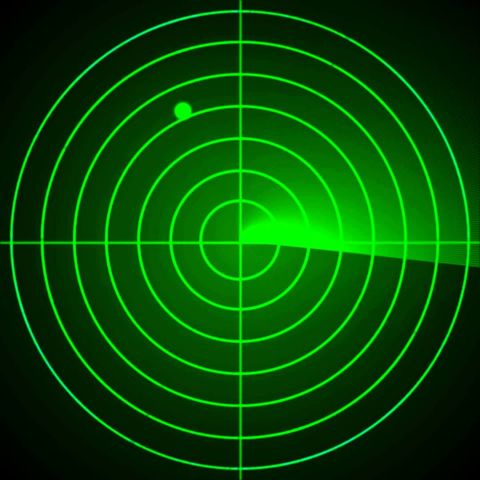
\includegraphics[width=2.5in]{radar.jpg}
	\end{figure}

	The radar engineers developed a way to look at this tradeoff, which is
	still popular to this day in machine learning. After training the
	logistic regression model (so we have $h\in\Hc_{logistic}^d$)  we make a grid of values of $\alpha$ in
	$[0,1]$. For each value of $\alpha$ we create a classifier by thresholding  $h$ at
	$\alpha$, and calculate the number of  Type-I and Type-II errors the
	classifier makes - preferably over a test sample that was not used for
	training the logistic regression (why?).  We plot a parametric curve of TPR (true
	positive rate) against FPR (false positive rate) when $\alpha$ is the
	parameter. This curve is called the {\bf Receiver Operating
	Characteristic (ROC)} curve. It is continuous, increasing and goes from
	$(0,0)$ in the FPR-TPR plane 
	(for $\alpha=0$ we classify everything as negative, so no false
	positives and not true positives) to $(1,1)$ (for $\alpha=1$ we
	  classify everything as positive, so false positive rate is $1$ - we
	  make every possible Type-I error - and
	  also true positive rate is $1$ - we ``catch'' all the positive
	samples).

	\begin{figure}[h!]
	  \centering
	  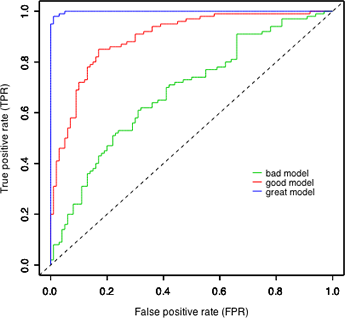
\includegraphics{roc.png}
	  \caption{ROC curves of three trained models (source:jxieeducation.com)}
	\end{figure}

	Convince yourself that if the ROC curve is a linear line from $(0,0)$ to
	$(1,1)$, the classifier is just a random guess. If a classifier has an
	ROC curve that is closed to this linear line, it's a poor classifier.
	Now convince yourself that if the ROC curve rises sharply from $(0,0)$,
	for example makes a ``jump'' to $(FPR=0.1, TPR=0.9)$, it's a good
	classifier - we are able to correctly detect $0.9$ of the positive
	samples at the price of $0.1$ false positive rate. 

	Plotting the ROC curve of a classifier has a few different uses:
	\begin{itemize}
	  \item {\bf Tuning $\alpha$.} It allows us to see the tradeoff, provided by the classifier,
	    between Type-I errors and correct detection of positive samples, so
	    we can choose the tuning of $\alpha$ we would like to work with for
	    the actual prediction - for using logistic regression  to actually
	    classify new samples.
	  \item {\bf AUC - a performance measure for the tradeoff itself}. 
	    It allows us to define a performance measure for the logistic
	    regression classifier known as {\bf Area Under the Curve} (AUC).
	    This performance measure evaluates the prediction rule $h$ we chose
	    without having to decide on $\alpha$ - it measures the quality of
	    the {\bf tradeoff} provided by $h$, a tradeoff from which we must
	    choose a specific point in order to actually classify new samples.
	    AUC is simply the {\bf definite integral} of the ROC curve on 
	    the segment $[0,1]$ - the area under the AUC curve. As mentioned
	    above, AUC around $1/2$ means that $h$ is poor - more specifically,
	    that the {\bf tradeoff} provided by $h$ is poor. AUC is bounded from above by $1$,
	    so an AUC close to $1$ means $h$ offers an excellent trade-off, and
	    in this case
	    we expect to be able to find a cutoff $\alpha$ that gives a
	    classifier with very few false-positives and very high detection
	    rate (true positive rate).
	  \item {\bf Comparing candidate rules.} Suppose that we have two or
	    candidate rules $h_1,h_2$ (or more). For example, maybe we trained
	    logistic regression on the same training sample with different
	    features, or maybe we have one rule that comes from logistic
	    regression and a different rule (that also gives estimated class
	    probabilities), and we're wondering which one to use. Now we have a
	    problem - we can't turn $h_i$ into an actual classification rule
	    without choosing a cutoff $\alpha_i$, but would like to compare
	    $h_1$ to $h_2$ without committing to a cutoff - to compare the
	    tradeoff offered by $h_1$ to that offered by $h_2$. It is very
	    useful here to plot the two ROC curves of $h_1$ and $h_2$ on a
	    single axis - and visually compare the tradeoffs they offer. 
	\end{itemize}



	As you've probably understood, the need to choose a threshold $\alpha$
	and the ROC curve are {\bf not} special to
	logistic regression. We need to choose $\alpha$, and can plot ROC curve,
	for any classification algorithm that produces ``estimated class
	probabilities'' rather than class predictions in $\left\{ 0,1
	\right\}$.


\subsection{Summary}
\begin{itemize}
  \item Hypothesis class: 
    \[
	\Hc_{logistic}^d= \left\{ \VV{x} \mapsto \pi(\innerr{\VV{x}}{\VV{w}} ) \right\}\,.
      \]

     \item Learning principle for training model (choosing $f\in\Hc$): Maximum Likelihood 
    \item Computational implementation of learning principle: Specialized
      iterative method based on Netwon-Raphson
      iterations, or a general convex solver
      (pay attention to effective rank of regression matrix -
      just like in linear regression. Near-singular regression matrix $X$ will
    cause numerical problems.)
  \item How to make predictions on new samples: with $\VV{w}$ the fitted weight
    vector:
    \[\hat{y} := \begin{cases} 1 & \pi(\innerr{\VV{x}}{\VV{w}})>\alpha \\ 0 &
    \pi(\innerr{\VV{x}}{\VV{w}}) \leq \alpha \end{cases}\,,\]
    where $0<\alpha<1$ is a {\bf cutoff} chosen to give a good tradeoff between
    false positive rate and true positive rate (a point on the ROC curve).
  \item Interpretable: Yes - using fitted regression coefficients
    \item Estimates class probabilities: Yes
  \item Family of models: Yes, as we add or remove features from regression
    matrix $X$. Also possible to add {\bf regularization} to control
    bias-variance for a fixed regression matrix $X$ - see future lectures. 
     \item Time complexity for training, and for predicting on a new sample:
  \item How to store trained model: store the regression weight vector $\VV{w}$ 
  \item When to use: Always try this, especially when classes are more or less
    balanced
\end{itemize}


\section{Nearest Neighbors}

And now for something completely different. {\bf Nearest neighbor}
classification is a popular, simple, effective learner that's simple to
understand - but (depending on the dimension and training sample size) may not so easy to implement. 
It is sometimes surprisingly
effective. And it is very different from all the other methods in this lecture.

\subsection{No hypothesis class}

Wait, what? 
Yes, this classifier is {\bf not} based
on our paradigm of hypothesis class, learning principle, and all that. {\bf A nearest
neighbor classifier has no training stage.} 

Every other classification algorithm in this lecture has an hypothesis class,
and a training stage in which we use the training sample $S$ to choose
some $h_S\in\Hc$. {\bf After the training stage, we can in principle discard  the
training sample} and just store the chosen hypothesis $h_S$ in order to make
predictions on new samples. 

Nearest neighbors classifiers are different. There is no hypothesis class and no
training stage. We must keep the entire training sample $S$ to make new
predictions: the algorithm just tells us how to use $S$ to make a prediction on
a new sample. 

\subsection{Prediction with $k$-nearest neighbors}

The algorithm need two parameters: an integer value $k$, and a distance function
$\rho$ on $\reals^d$. We can use the square Euclidean norm $\rho(\VV{x},\VV{z}) = 
\norm{\VV{x}-\VV{z}}$. Or we can use a {\bf weighted} square norm that gives more
importance to some features: $\rho(\VV{x},\VV{z}) = \sum_{j=1}^d \omega_j
(x_j-z_j)^2$, for some fixed weight vector $(\omega_1,\ldots,\omega_d)$ and
where $x_j$ is the $j$-th coordinate of the vector $\VV{x}\in\reals^d$. 
 \\~\\
So, what's the algorithm? Let $S=\left\{ (\VV{x}_i,y_i) \right\}_{i=1}^m$ be our
training sample and let $\VV{x}$ be the test sample we wish to classify. 

The algorithm finds the $k$ training samples closet (with respect to the
distance $\rho$ provided) to $\VV{x}$ and predicts by majority vote of the labels
of  these $k$ (training samples) 
nearest neighbors.

Formally, 
\begin{itemize}
  \item Let $\pi = (\pi_1,\ldots,\pi_m)$ be a permutation of $(1,\ldots,m)$ such
    that \[\rho(\VV{x},\VV{x}_{\pi(1)}) \leq \rho(\VV{x},\VV{x}_{\pi(2)}) \leq
    \ldots \rho(\VV{x},\VV{x}_{\pi(m)})\,.\]
    So that $\VV{x}_{\pi(1)} ,\ldots,\VV{x}_{\pi(k)}$ are the
    $k$-nearest-neighbors of $\VV{x}$ among the samples in $S$, with respect to
    the distance distance $\rho$. 
  \item The predicted class is 
    \[
      \text{argmax}_{y\in\left\{ 0,1 \right\}}
    \sum_{ i=1}^k\mathbf{1}_{y_{\pi(i)}=y}
    \]
\end{itemize}

\subsection{Choosing $k$}
In fact, nearest-neighbors is a family
of learning algorithms, one for each $k$. 
The possible values
for $k$ are between $1$ ($1$-nearest-neighbor) and $m$. 

What happens at the extremes $k=1$, $k=m$?
\begin{itemize}
  \item 
    When $k=1$, the test point just copies the label of its nearest neighbor in the
training set. The decision boundaries are known as {\bf Voronoi cells}. The
classifier has very low bias and very high variance (why?)

\begin{figure}[h!]
  \centering
  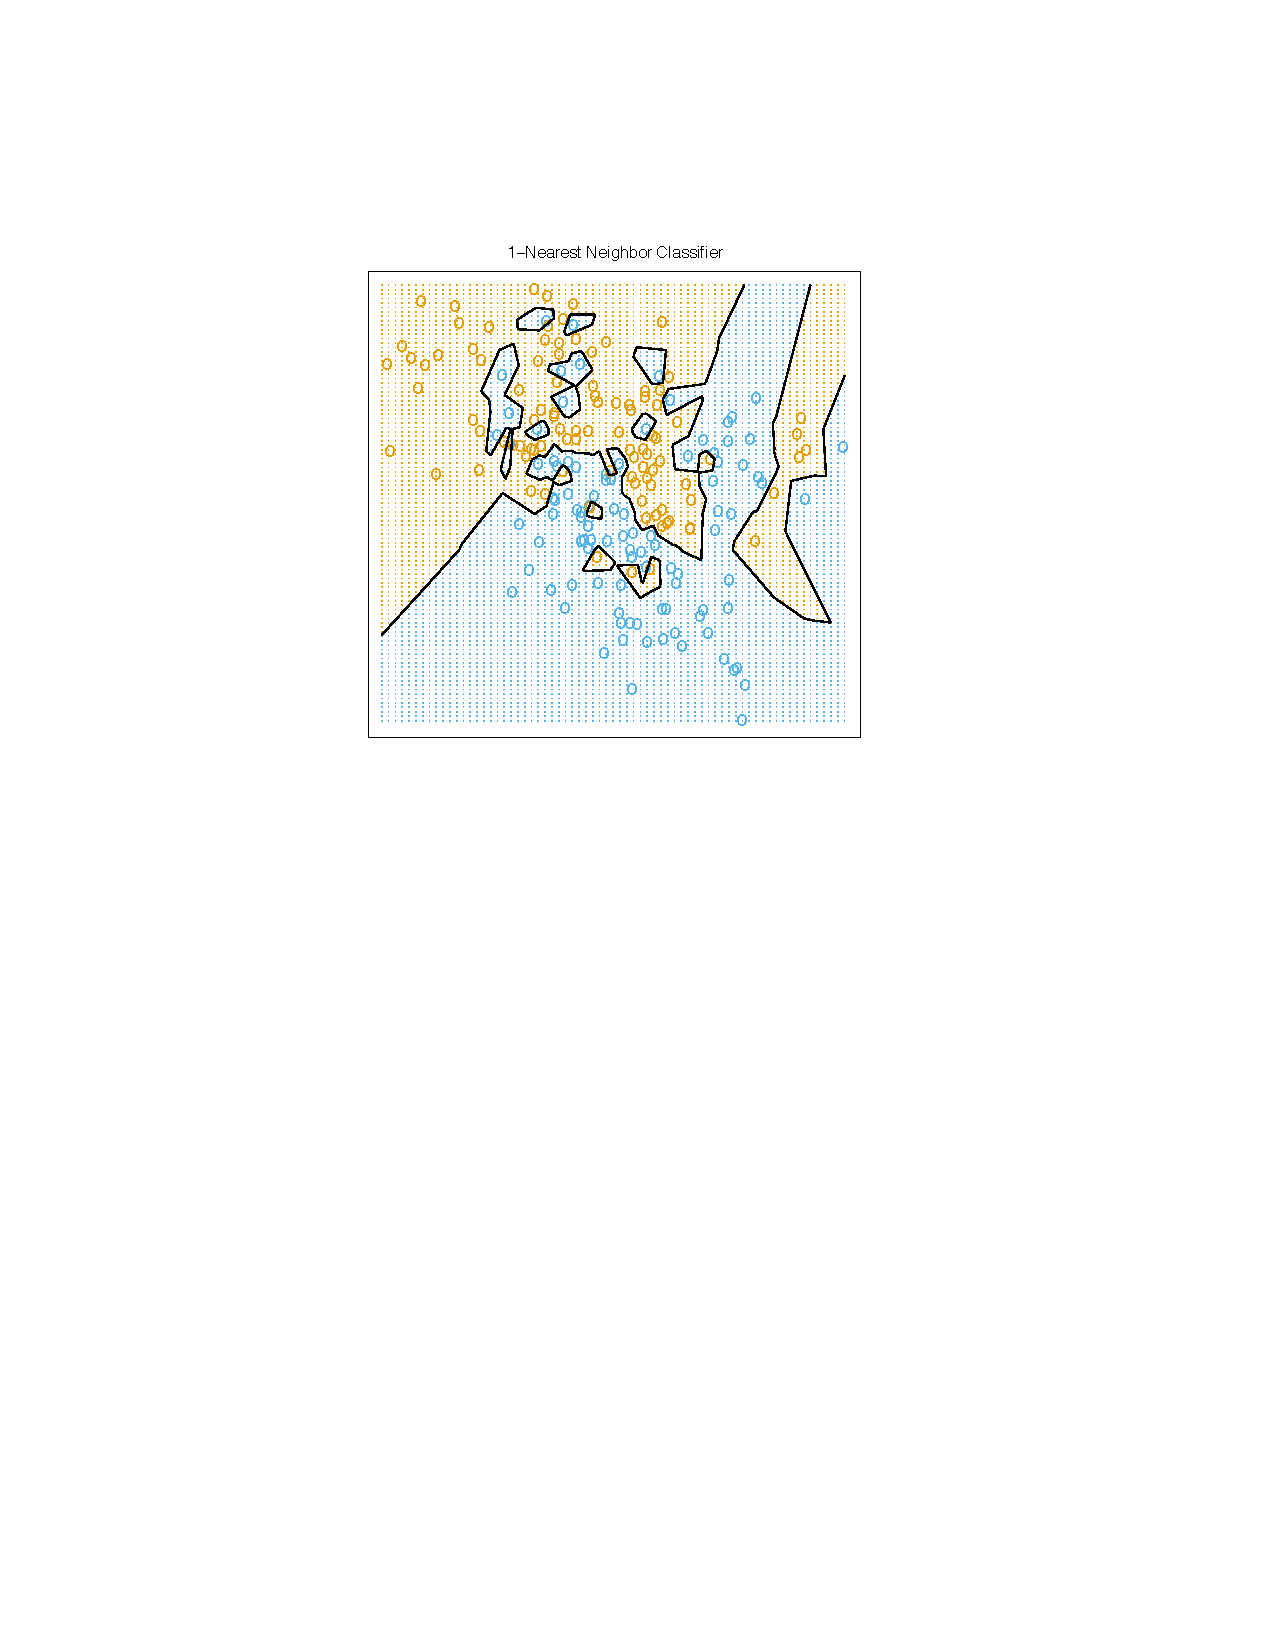
\includegraphics{esl_1_nn.pdf}
  \caption{Decision boundary for a $1$-NN classifier (source: ESL)}
\end{figure}

\item When $k=m$, the classifier predicts a single class for every point in
  $\reals^d$ - the majority vote of all the training sample. Bias is (very,
  very) large, variance is zero. 
\end{itemize}

And in less extreme values of $k$, what do we get?
\begin{itemize}
  \item 
    When $k=3$ (say) the prediction is a majority vote of the 3 nearest
    neighbors of the test sample. (It's good to take an uneven $k$ so that there
    will always be a majority vote.) 
The
classifier has low bias and high variance. To see why, think how many training
samples will need to change their class labels in order for a test sample to
receive a different prediction. If the vote for some test sample is 2-1, it's
enough that {\bf one} test sample will change its label, and the prediction will
change. 

\item When $k=m/3$ (say)  the prediction is a majority vote of {\bf a third} of the
  training sample points. The classification rule is constant on large parts of
  $\reals^d$. Bias is high, variance is low. (Again, think how many training samples
  need to change their class for the prediction to change.) 

  \begin{figure}[h!]
  \centering
  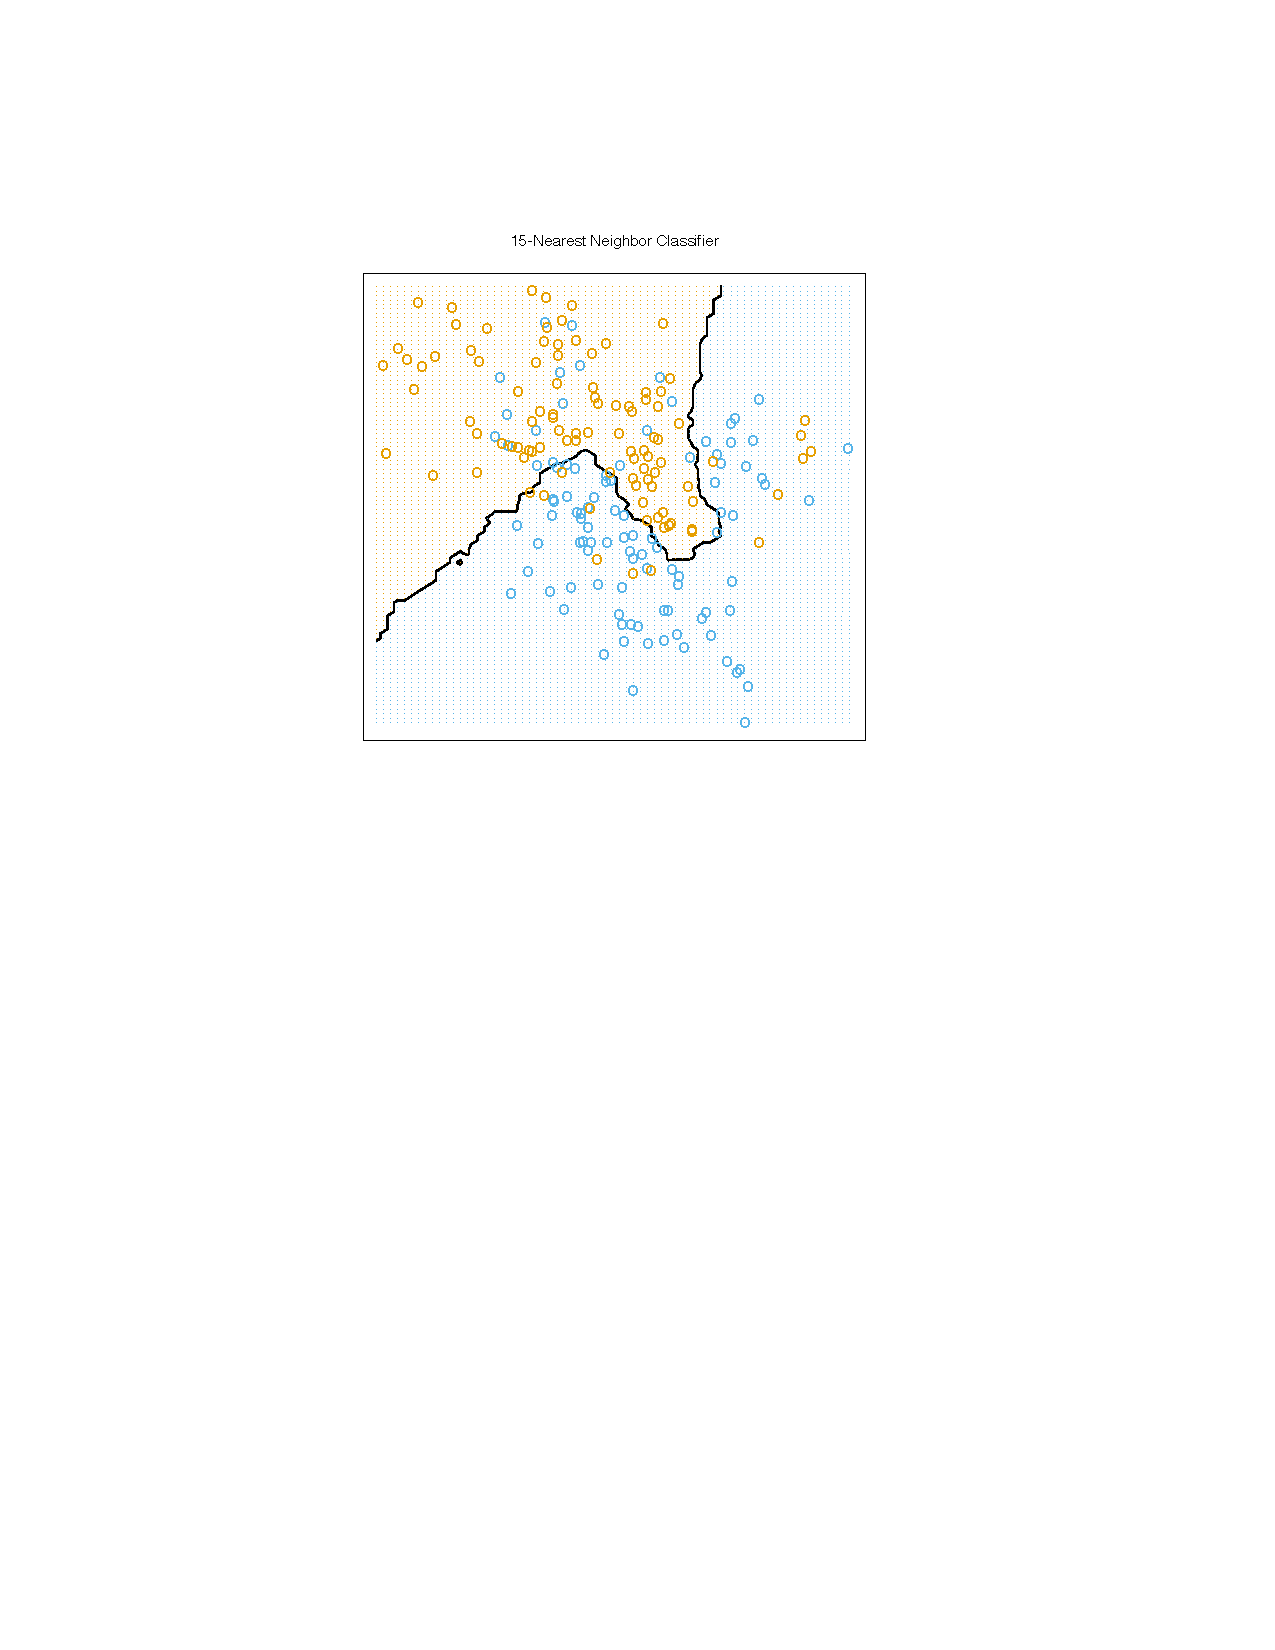
\includegraphics{esl_15_nn.pdf}
  \caption{Decision boundary for a $15$-NN classifier (source: ESL)}
\end{figure}

\end{itemize}

As we change $k$ we change the bias-variance tradeoff. Typically we will see
something like this for the test error of a $k$-NN classifier, as
misclassification error is plotted over $k$:

 \begin{figure}[H]
  \centering
  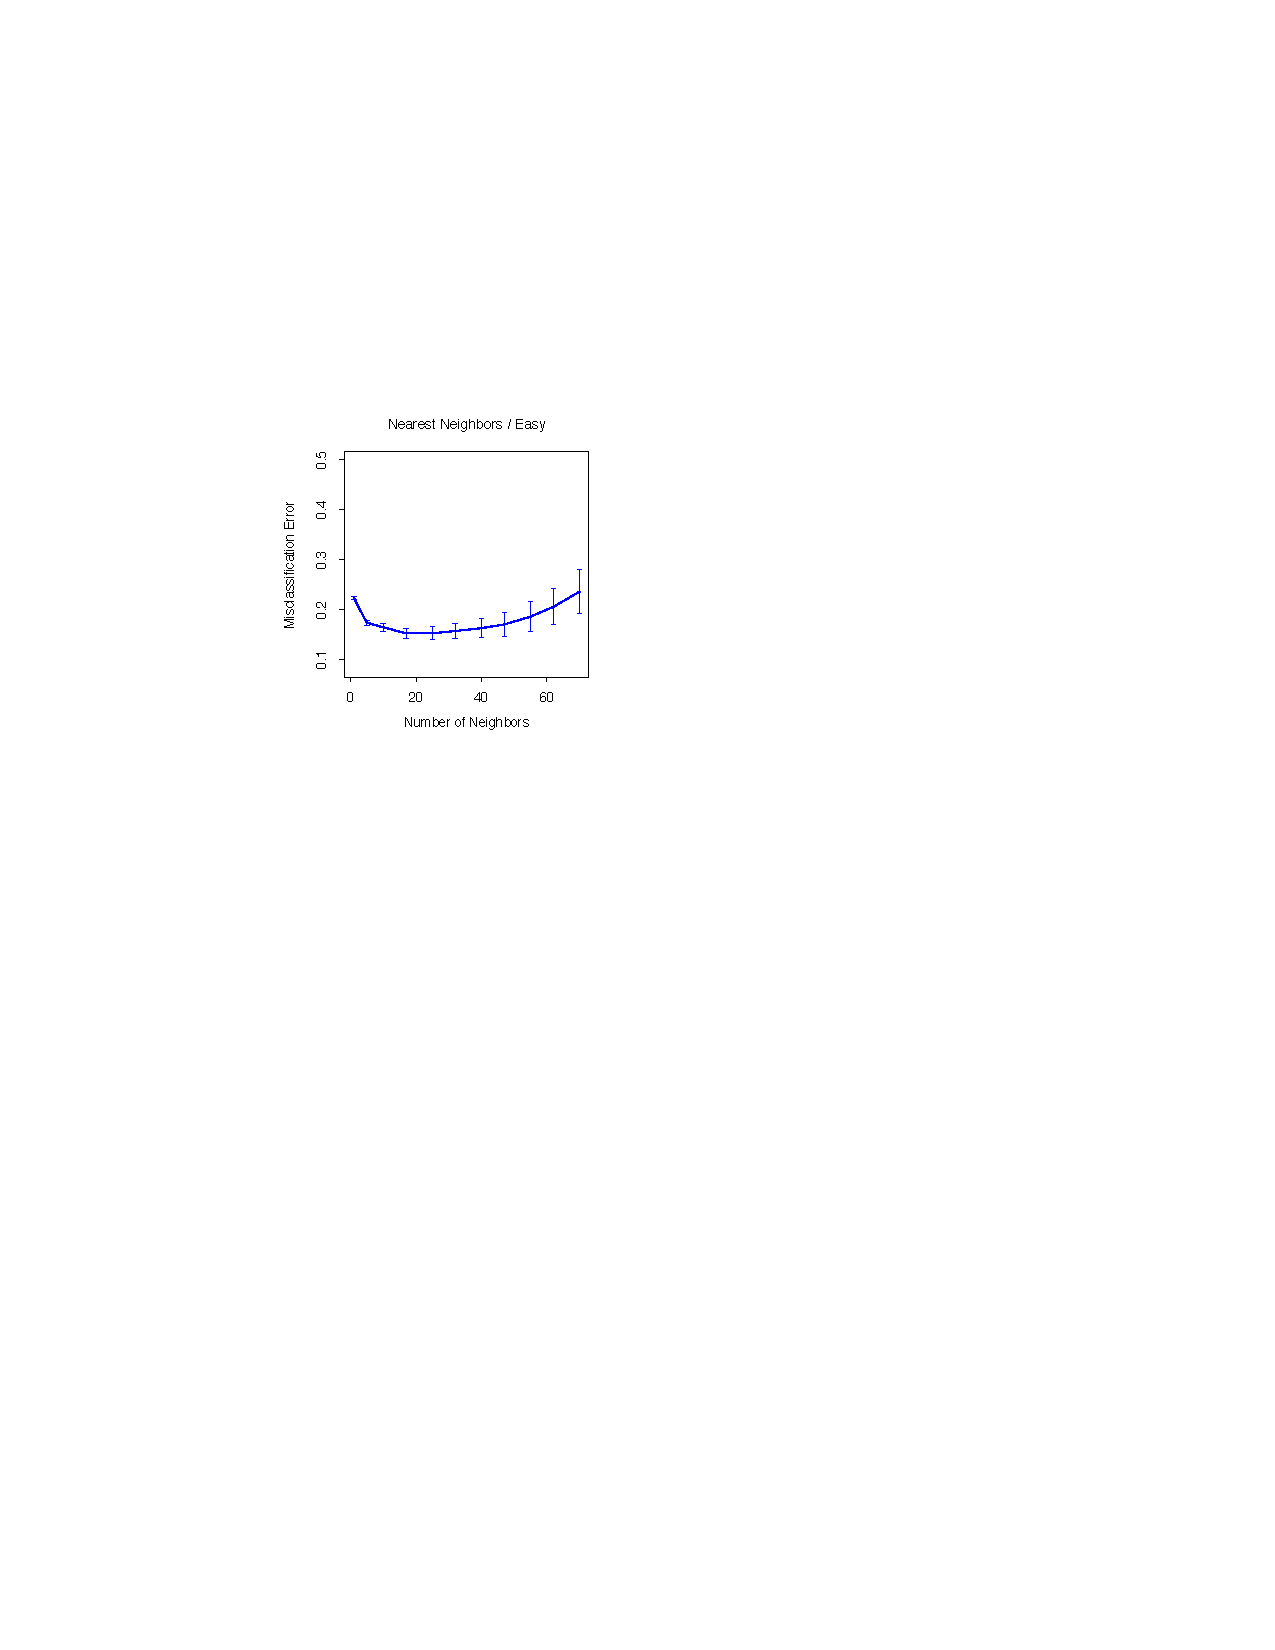
\includegraphics[width=3in]{esl_nn_vary.pdf}
  \caption{Test error of a $k$-NN classifier over $k$ (source: ESL)}
\end{figure}


We will talk about this in more detail later in the course. This is an example
of the {\bf general phenomenon} for most learning algorithms, which we have mentioned several times before: 

 \begin{figure}[h!]
  \centering
  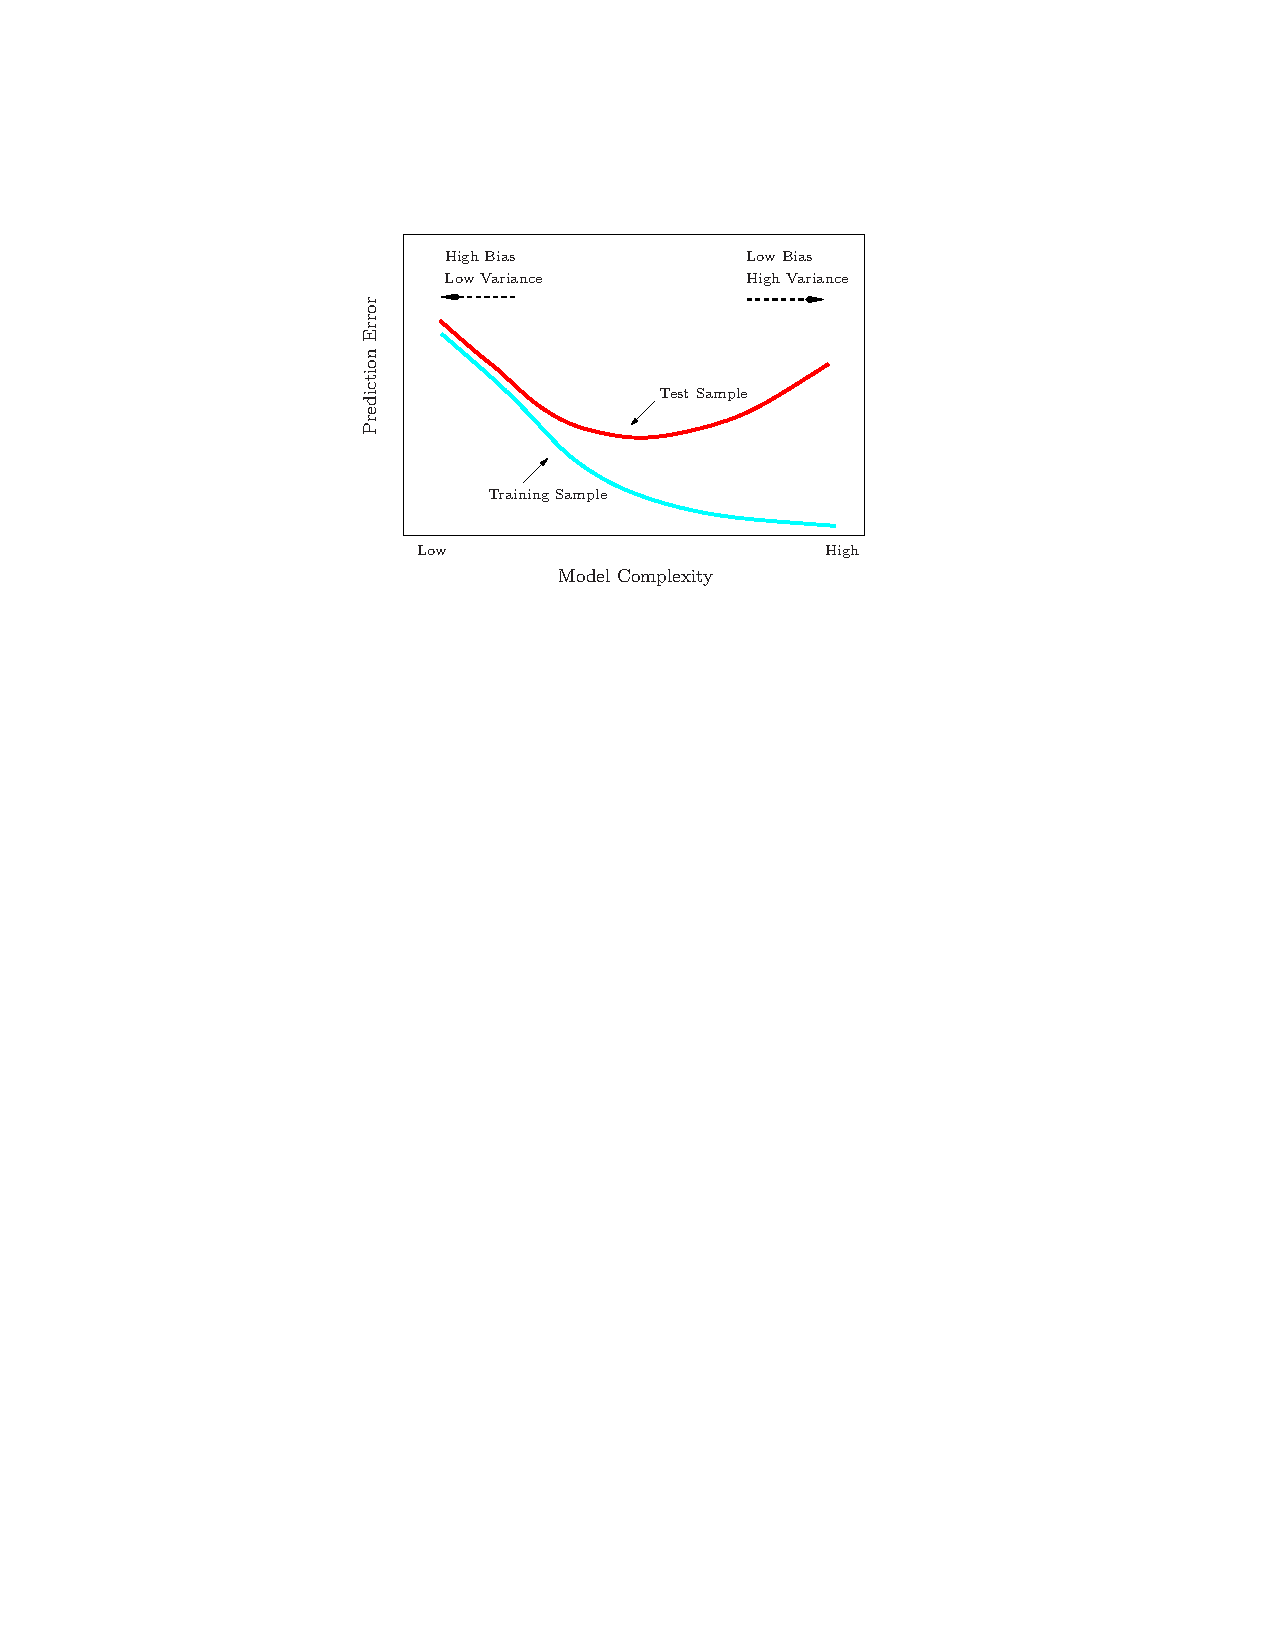
\includegraphics[width=4.5in]{ESL_bias_variance.pdf}
  \caption{General shape of a bias-variance tradeoff (source: ESL)}
\end{figure}


\subsection{Computational implementation of $k$-nearest neighbors}

Implementing a $k$-nearest-neighbors classifier is very easy on small datasets,
and not so easy when the dimension $d$ and/or the sample size $m$ are large.
There are generally three types of implementation approaches:

\begin{itemize}
  \item {\bf Brute force implementation}: We keep the entire training sample $S$
    in storage during the entire prediction process. For each new test sample
    $\VV{x}\in\R^d$, we calculate $\norm{\VV{x}-\VV{x}_i}$ for all $1\leq i\leq
    m$ and partially sort to find the $k$ smallest distances. (What's the time
    complexity? And how much space is needed?)
  \item {\bf Exact nearest neighbors search with preprocessed data structure}:
    If $\rho$ is the Euclidean norm,
    algorithms such as {\tt kd-tree} and others can be used to pre-process the
    training sample and construct a {\bf special data structure}. (This is kind of a
      training stage, even though we don't come up with a hypothesis, just
      cache computations regarding the training sample so our prediction will be
    faster.) We don't need to keep the training sample $S$, just the data
    structure. Then at prediction time the data structure is used to quickly
    locate the $k$ nearest neighbors of the test sample $\VV{x}$.
  \item {\bf Fast randomized nearest neighbors search}: 
    beyond our scope in this course.
\end{itemize}



\subsection{Other sample spaces}

Nearest neighbors is the only classification algorithm we learn in this lecture,
which can work on sample spaces other than $\X=\reals^d$. Indeed, we just need a
distance function $\rho$ on $\X$. The implementation may be challenging, as all
the tricks that are available to speed up computation in $\R^d$ are not
available generally. 

\subsection{Summary}
\begin{itemize}
  \item Hypothesis class $\Hc$: None (``model free'')
  \item Learning principle for training model (choosing $f\in\Hc$): none - no model
  \item Computational implementation:
    Brute force nearest neighbor search; 
    kd-tree and similar exact methods which speed up prediction on new samples; 
    fast randomized nearest neighbors 
  \item How to make predictions on new samples: if using brute force, calculate
    distance to every point in sample 
  \item Interpretable: No
    \item Estimates class probabilities: No (unless using with many neighbors)
    \item Family of models: Yes, according to $k$ (using $k$-nearest neighbors)
     \item Time complexity for training, and for predicting on a new sample:
     \item How to store trained model: no trained model. Must store the entire
       training sample $S$ (or preprocessed data structrue)
     \item When to use: Always try when implementation possible. Especially when you're out of ideas.
\end{itemize}


\section{Classification Trees}
 

One of the most useful algorithms for classification {\bf and} regression known is the {\bf CART Random
Forest.} CART stands for Classification and Regression Trees. A random forest,
is, well, a large collection of trees. 
Over a few lectures, we will to develop the full CART Random
Forest algorithm in three steps:
\begin{enumerate}
  \item {\bf Growing the classification tree} (A regression tree is very similar
    - if you understand classification trees you understand regression trees.)
  \item {\bf Pruning the tree} using a regularization principle for precise control
    over bias-variance tradeoff.
  \item {\bf Bagging trees} to create a random forest.
  \end{enumerate}

  As we will see,  are different ways to {\bf grow} and {\bf prune} a
  classification tree. We will see a method for growing and pruning called CART.
  This lecture will focus on the first step. We'll see {\bf pruning} and {\bf bagging} in later lectures.
 
  So let's grow a CART classification tree. It is an interesting classifier in and of itself,
  but the real reason to learn it is to understand the much more powerful (and
  popular) Random
  Forest classifier. 

  In this section we'll use the label set $\Y=\left\{ 0,1 \right\}$.

  \subsection{Tree-induced,  axis-parallel partitions of $\reals^d$}

 We've already seen two classifiers that use piecewise-constant prediction
 rules: half-spaces and SVM. In both the hypothesis class is a half-space, where
 we predict class $1$ (say) on one side of a hyper-plane, and $0$ (say) on the
 other side. 

 Now we would like to use more complicated piecewise-constant prediction rules
 (more complicated hypotheses.) Let's consider a rule that partitions the
 sample space $\reals^d$ into {\bf axis-parallel boxes, or ``hyper-rectangles''}, and it each
 box we predict either $1$ or $-1$. The learner's task would be to use the
 training sample to 
 ``chop'' the sample space $\X$ into a disjoint union of axis-parallel boxes, and
 to assign a class prediction to each box. 

 To make our hypothesis class a little smaller and a little simpler, let's focus
 on  disjoint unions of boxes that are obtained by iteratively chopping an
 existing box into two smaller boxes along one of the axes. More specifically:
 \begin{itemize}
   \item We start with the whole sample space $\reals^d$
   \item We chop $\reals^d$ into two axis-parallel ``boxes'' (a half-space is
     also a box in our terminology) by selecting one of the $d$ coordinates, say
     the coordinate $i_1$
     ($1\leq i_1 \leq d$) and a value $t_1\in\reals$. The two boxes will
     be $B_+=\left\{ \VV{x}\in\reals\,|\, x_{i_1}>t_1 \right\}$ and 
     $B_-=\left\{ \VV{x}\in\reals\,|\, x_{i_1}\leq t_1 \right\}$.
     When then chop $B_+$ by again selecting a coordinate $i_{2,1}$ and a value
     $t_{2,1}$ (such that $t_{2,1}>t_1$ so we are chopping inside the box $B_+$)
     and Define $B_{++} = \left\{ \VV{x}\in B_+\,|\, x_{i_{2,1}}>t_{2,1} \right\}$
     and  $B_{+-} = \left\{ \VV{x}\in B_+\,|\, x_{i_{2,1}}\leq t_{2,1}
     \right\}$.
     Similarly we choose a coordinate $i_{2,2}$ and a value $i_{2,2}$ and chop
     $B_-$ into  $B_{-+}$ and  $B_{--}$. Now we have $\reals = B_{++} \biguplus
     B_{+-} \biguplus
     B_{-+} \biguplus
     B_{--} $. We can stop here, or we can chop any (or all) of the existing
     boxes into smaller axis-align boxes. We may, for example, choose to only
     chop $B_{++}$   further, and leave the others as they are. 
     Finally we stop chopping, and are left with a partition of $\reals$ into a
     disjoint union of axis-aligned boxes. We call such a partition a Tree
     Partition. 
     
     \begin{figure}[h!]
       \centering
       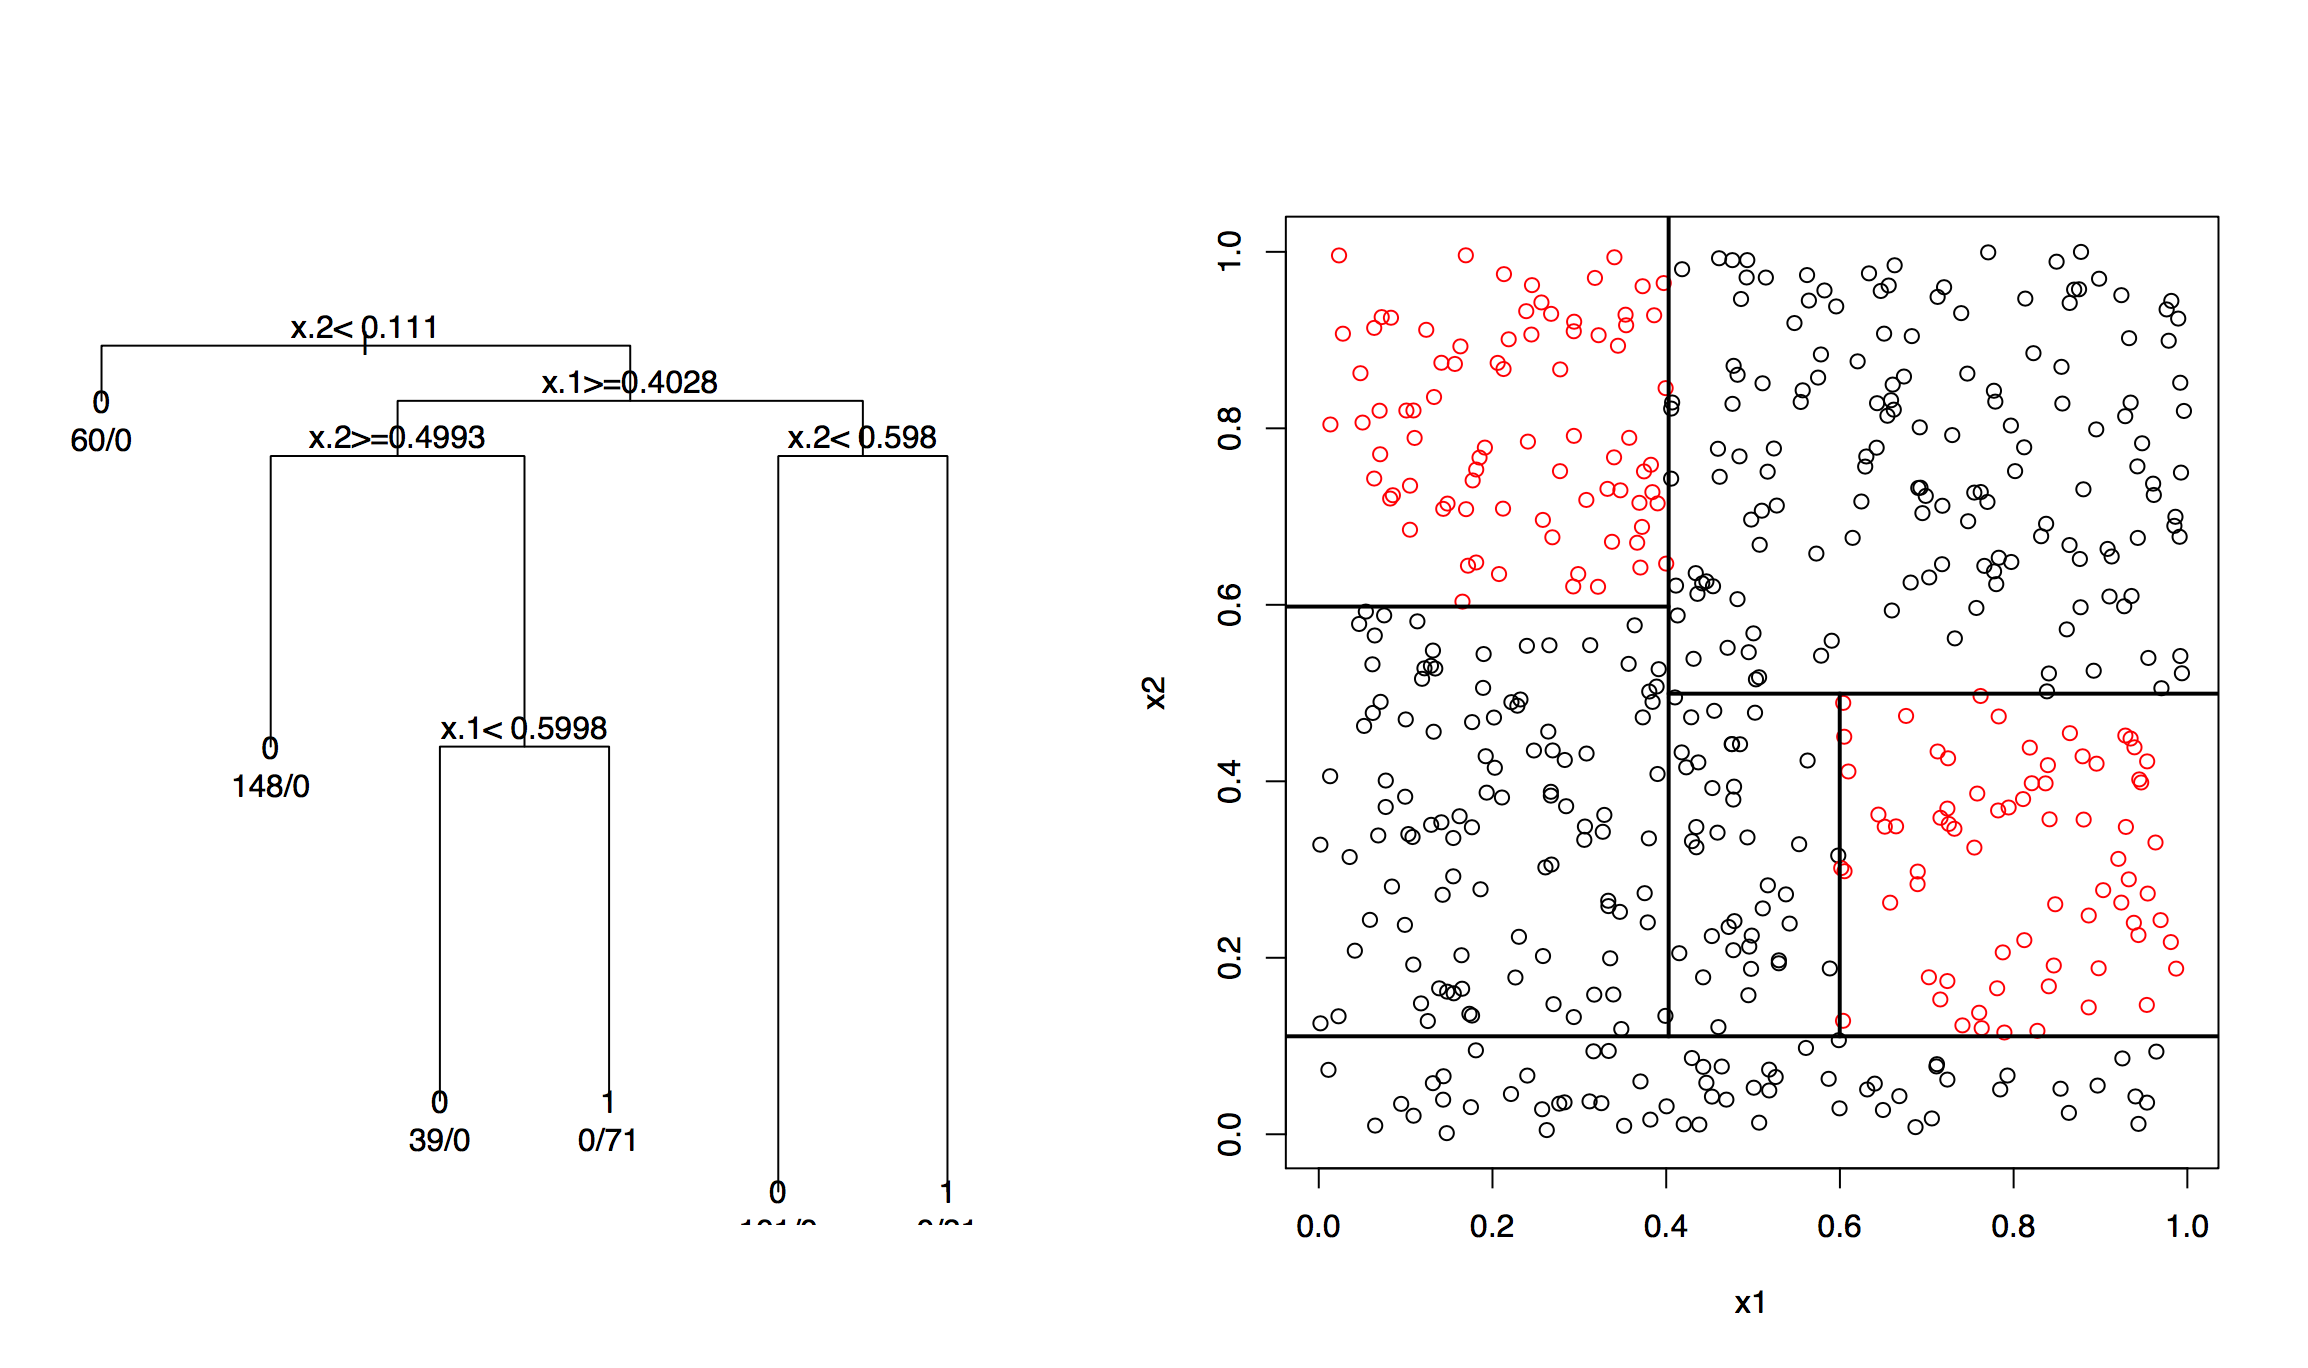
\includegraphics[width=5in]{tree2.png}
       \caption{A tree and its induced partition in $\R^2$}
     \end{figure}
     
     Note that the partitions obtained
     this way are special - most partitions of $\reals^d$ into axis-aligned
     boxes are not Tree Partitions, namely, cannot be constructed by such a
     top-down iterative chopping procedure. 

      \begin{figure}[h!]
       \centering
       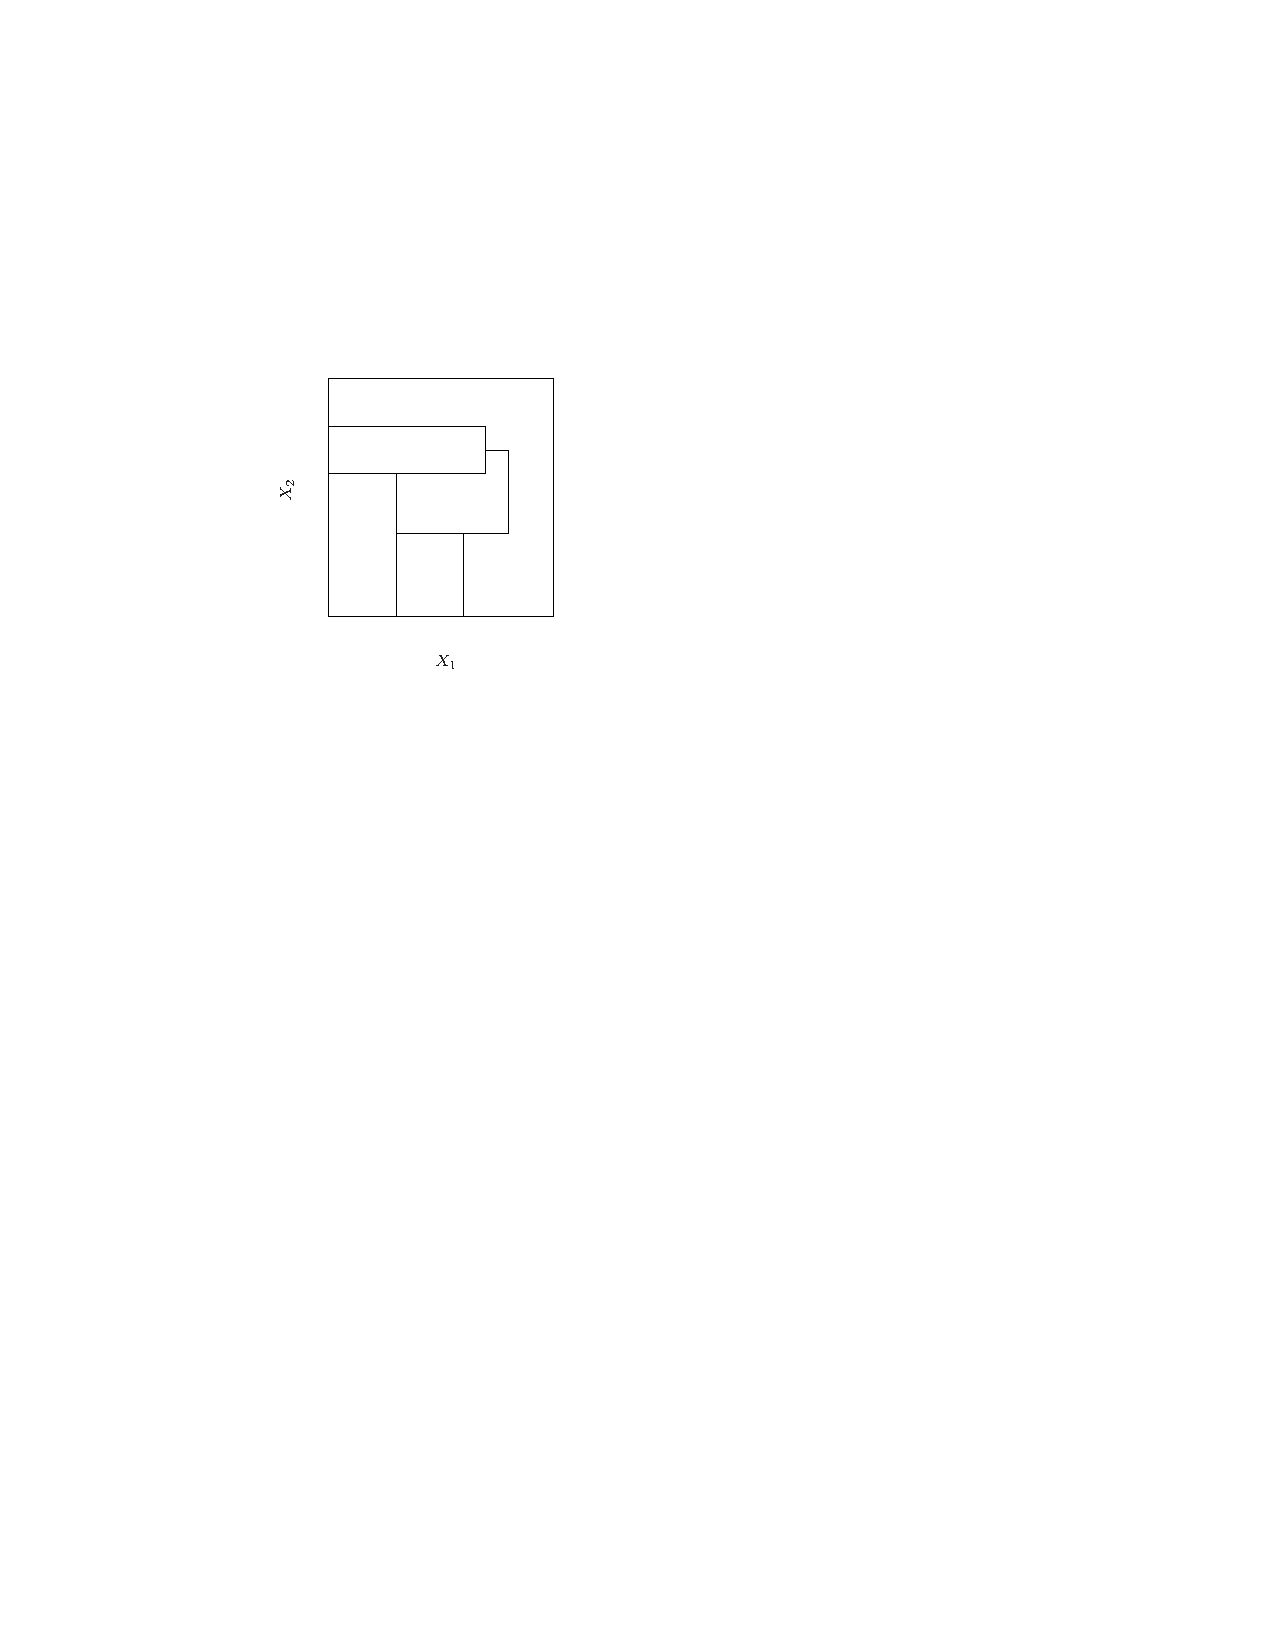
\includegraphics[width=3in]{esl_no_tree.pdf}
       \caption{A partition into axis-aligned boxes that is {\bf not} a tree
       partition. (Source: ESL)}
    
     \end{figure}

    
     \subsection{The Regression Tree hypothesis class}

     The hypothesis class $\Hc_{CT}$ we will consider consists of piecewise-constant
     functions, that assign a class prediction ($1$ or $0$) to each box in a
     Tree Partition. Unless we restrict it somehow, the class contains all
     piecewise-constant functions supported on all Tree Partitions of $\reals^d$
     (to any number of boxes).
     Formally, for a Tree Partition $\reals^d=\biguplus_{j=1}^N B_j$ of
     $\reals^d$ into $N$ boxes, and label assignments $c_j \in \left\{ 0,1
     \right\}$ ($j=1,\ldots, N$) assigning label $c_j$ to box $B_j$, the
     hypothesis $h\in\Hc_{CT}$ is a function $h:\reals^d\to\left\{ 0,1
     \right\}$ defined by 
     \[
       h(\VV{x}) = \sum_{j=1}^N c_j \mathbf{1}_{B_j}(\VV{x})
     \]
     where $\mathbf{1}_{B_j}$ is the indicator function of $B_j$. 

     \subsection{Any hypothesis in $\Hc_{CT}$ corresponds to a Decision Tree,
     and vice-versa}
    
     Let's talk about something else for a second, which we turn out to be
     closely related to the hypothesis class $\Hc_{CT}$ we just defined.

     Outside computer science and machine learning, there is a time-honored way
     to classify, or to {\bf make decisions.} Suppose someone comes into a
     hospital emergency room. The first step of triage is to determine - fast - whether
     they are in a life-threatening medical emergency, or else they can wait in
     line and receive treatment in a little while. The triage uses a sequence of
     yes/no questions, such as: 
       Is the patient conscious yes/no? \\
	   - If not conscious: Classify as {\bf emergency}\\
	   - If yes conscious: Is the patient's pulse $<40$ beats per
	     minute?
	     \begin{itemize}
	       \item If yes, pulse $<40$: Classify as {\bf emergency} 
	       \item If no, pulse $>40$: Is the patient's pulse $>130$ beats per
		 minute?
		\begin{itemize}
	       \item If yes, pulse $>130$: Is the patient's systolic blood
		 pressure $<80 mm Hg$?
		 \begin{itemize}
		   \item If yes, blood pressure $<80 mm Hg$,  classify as {\bf
		     emergency} 
		   \item If no, blood pressure $>80 mm Hg$: Is the patient's systolic blood
		 pressure $>140 mm Hg$?\\
		 - If yes, blood pressure $>140 mm Hg$, classify as {\bf
		     emergency} \\
		 - If no, blood pressure $<140 mm Hg$, classify as {\bf
		     not emergency} 
	     \end{itemize}

	       \item If no, pulse $<130$: classify as {\bf not emergency}
	     \end{itemize}
	     \end{itemize}
 \end{itemize}

 This is a {\bf decision tree} that uses three features: {\bf conscious} (a
 binary categorical feature), {\bf pulse} (a numerical feature) and {\bf blood
 pressure} (also a numerical feature). See if you can we write a diagram for
 this decision tree in the shape of a tree, where every node is a question, and
 every leaf is a decision / classification. The root of the tree is the first
 question (``conscious yes/no?'').

 Now observe that {\bf every function in our Classification Trees 
   hypothesis class  $\Hc_{CT}$ is
 equivalent to a decision tree}. In the notations  of the generic example above, 
 the first question is: ``$x_{i_1} > t_1$ - yes/no?''; If yes, we ask the second
 question ``$x_{i_{2,1}} > t_{2,1}$ - yes/no?''. If no, we ask the second question
 ``$x_{i_{2,2}} > t_{2,2}$ - yes/no?''. And so on, until there are no more splits and we
 have reached a box over which 
 the function in $\Hc_{CT}$ is constant. If the constant value is $+1$, we
 classify / predict class $1$. If the constant value is $0$, we predict class
 $0$. 

 This is why our hypothesis class is called - classification {\bf trees}.

 \subsection{How {\em not} to grow a classification tree}

 Having defined our hypothesis class, the next question is of course - what
 learning principle shall we use, namely, how shall be select $h_S\in\Hc_{CT}$
 based on a training sample $S$. We have to work with some loss - for example,
 let us work with misclassification loss - simply counting misclassifications.
 But as you will see, in what follows you can replace this  loss with any other
 loss function you prefer. 

 Let's start from the end. Suppose that we have already somehow 
 decided to use a certain Tree Partition of $\reals^d$ that consists of $N$ disjoint boxes,
 $\reals^d=\biguplus_{j=1}^N B_j$. Let $S=\left\{ (\VV{x}_i,y_i)
 \right\}_{i=1}^m$ be our training sample.
 %Define 
% $ n_j := \big|  \left\{ 1\leq i \leq m| \VV{x}_i\in B_j \right\}\big|$. 
 %(the number of training samples that fall inside the box $B_j$). 
 If the predicted
 label assigned to box $B_j$ is $\hat{y}(B_j)\in\left\{ \pm 1 \right\}$ then 
 the number of misclassification errors that are incurred by the training
 samples that fall inside $B_j$ is of course $\sum_{ \VV{x}_i\in B_j
 }\mathbf{1}_{y_i\neq\hat{y}(B_j)}$. Let's apply the ERM principle - and try to
 minimize the misclassification errors on our training set. 
 
 For any box $B$ in a tree partition, and a sample $S=\left\{ (\VV{x}_i,y_i)
 \right\}_{i=1}^m$, and a label $y\in\left\{ 0,1 \right\}$, define
\[
  P^S_y(B) := \frac{1}{n_S(B)}\sum_{ \VV{x}_i \in B
  }\mathbf{1}_{y_i=y}\,,
\]
where $n_S(B) = \big|  \left\{ 1\leq i \leq m| \VV{x}_i\in B \right\}\big|$ is
just the number of training samples in $S$ that fall inside the box $B$. 

 The label that will
 minimize the empirical risk for those training samples that fall inside the box
 $B$ is of course the {\bf majority vote} 
 \[\hat{y}_S(B) = \argmax_{y\in\left\{ 0,1
 \right\}} P^S_y(B)\]
 - checking which label has more samples inside $B$ - this
 is
 the label for which we make less misclassification errors inside the box $B$.


 So, adopting the ERM principle, the labeling assignment, for a given tree
 partition $\reals^d=\biguplus_{j=1}^N B_j$, the assignment that minimizes the
 misclassification for the training sample $S$ is given by labeling the box $B_j$
 with $\hat{y}_S(B_j)$.
 
 It follows that, for our training sample $S$, 
 for each Tree Partition there is a unique label assignment - and therefore a
 unique classification tree (hypothesis) $h\in\Hc_{CT}$ that minimizes the
 empirical risk. It seems, therefore, that all we have to do is look for the
 tree that minimizes ERM $h\in\Hc_{CT}$, namely find 
 \[
   \text{argmin}_{h\in\Hc_{CT}} L_S(h)
 \]
 where $L_S(h)$ is the misclassification error of the candidate classification
 tree $h$ on the training sample $S$.

 But wait. If we don't limit the number of levels of the tree, we know which
 tree will minimize the empirical risk - the tree with so many levels that each
 sample in $\VV{x}_i\in S$ finds itself alone in a box, and that box is (of course) labeled
 with the label $y_i$. Convince yourself that such a classification tree has
 empirical risk $L_S(h)=0$. But this tree won't generalize well to new samples.
 (Why? - this is the very definition overfitting: we used the fact that
   $\Hc_{CT}$ is very large to find $h\in\Hc_{CT}$ that fits the training sample
 $S$ {\bf exactly}. So our learner has huge {\bf variance}.)

 The solution? We should of course limit the number of levels in the
 classification tree. Let $\Hc_{CT}^k$ denote the hypothesis class of
 classification trees with at most $k$ levels. Note that we now have {\bf a
 family of hypothesis classes} - one for each $k$ - not just one hypothesis
 class. Convince yourself that $k$ controls the size of the hypothesis class and
 therefore controls a bias-variance tradeoff:
 \begin{itemize}
   \item
 For small $k$,  $\Hc_{CT}^k$ is
 small, and therefore the ERM learner over  $\Hc_{CT}^k$, namely the learner
 that chooses $h_S\in\Hc_{CT}^k$ with the lowest empirical risk,  will have very high bias
 (only very simple functions on $\reals^d$ can be approximated by classification
 trees with just a few levels) and very low variance (the boxes are very large,
   so labels assigned to each box are based on majority vote of typically many
   training samples. So changing a few training samples will barely change the
 selected hypothesis $h_S$.)
 \item For large $k$,  $\Hc_{CT}^k$  is large, and therefore the ERM learner
   over  $\Hc_{CT}^k$ will have low bias (we can approximate even complicated
   functions on $\reals^d$ with classification trees with many levels), and high
   variance (the boxes are small, so labels assigned to each box are based on
     majority vote of typically just a few samples. So changing a few training
   samples could change the label assignment of many boxes.)
\end{itemize}

Ok, so it seems we have a solution: We will choose a reasonable value for $k$,
namely, select a specific hypothesis class among the family of all possible
classification tree hypothesis classes, and use ERM, namely return 
\[
  \text{argmin}_{h\in\Hc^k_{CT}} L_S(h)\,.
 \]


 \subsection{How to grow a classification tree}

 Houston, we have a problem. How do we find the minimizer
 $\text{argmin}_{h\in\Hc^k_{CT}} L_S(h)$ computationally? Namely, how do we
 implement the ERM principle over $\Hc^k_{CT}$? 
 So far, the examples we've seen of learners based
 on the ERM learning principle lead to computationally tractable problems:
 linear regression was based on ERM, and we had a closed form expression for the
 minimizer. Half-space classifier was based on ERM, and lead to a simple
 convex optimization problem. But now? the search space $\Hc^k_{CT}$ is large
 (how many different hypothesis are in $\Hc^k_{CT}$?) and has no
 Euclidean or other structure  that can be used. To find ERM, it seems we would
 have to use brute force search, which is infeasible. (In fact, one can prove
   that implementing ERM on  $\Hc^k_{CT}$ is an NP-hard problem with respect to
   the training sample size\footnote{By
     reduction from ``three-dimensional matching'', see
     Hyafil and Rivest, ``Constructing Optimal Binary Decision Trees is
   NP-Complete'', {\em Information  Processing Letters} {\bf 5}(1), 1976}. 

   What do we do? this is the first time that we come fact to face with the
   bitter truth that while the ERM principle is nice, it is often impossible to
   implement - especially when the hypothesis class on which we are working has
   no Euclidean structure. 

   So we must resort to {\bf heuristics}. This is where it gets interesting.
   While the definition of classification trees,  and of $\Hc^k_{CT}$, as well
   as how to assign prediction labels to boxes in a Tree Partition  given a
   training sample, are all canonical, there are several different heuristic
   approaches to how to proceed and ``grow a classification tree'' - namely,
   choose $h_S\in \Hc^k_{CT}$ - in practice. 

   One approach, that came out of the statistical learning community, is known
   as {\bf Classification and Regression Trees} (CART). It is described in
   detail in ``Elements of Statistical Learning 2nd ed.'' section 9.2. Another
   set of approach came out of the computer science machine learning community,
   are known by the weird names {\bf ID3}, {\bf C4.5} and {\bf C5.0}. The
 simplest of these, ID3, is described in ``Understanding machine learning''
 section 18.2. While these approaches differ in details, all of these are
 basically greedy heuristic that build a tree top-down and then ``prune'' it
 (merge some of the boxes back into larger boxes).

 Here, we will develop the CART heuristic, which is quite similar to C5.0, and has very well
 polished and efficient software implementation in software packages. 

 \subsection{Growing classification Trees a-la CART}

 CART consists of two stages: {\bf growing} the tree, which results in a tree
 that is a little too large, and then {\bf pruning} the tree to bring it down to
 the most effective size. We start with how to grow the tree and will discuss
 pruning in a later lecture. 
\\~\\
Suppose we chose $k$ to be the maximal tree depth (we will discuss how to choose
$k$ in a later lecture). The heuristic to grow a full classification
tree with at most $k$ levels will proceed top-down, starting from $\reals^d$ and
progressively chopping each box into two boxes. We don't chop a box under one of
two conditions: (i) the maximum number of levels $k$ has been reached; or (ii)
the box has reached a minimal number of training samples that was
pre-determined. (As we will see, it makes no sense to chop a box with very few
training samples in it.) If no minimal number of sample was specified, we anyway
have to stop if a box only has one training sample. 
Each existing box $B$ is chopped into two
boxes as follows:


\begin{itemize}
  \item for each coordinate $i\in\left\{ 1,\ldots d \right\}$, and each
    potential chopping value $t\in\reals$, let $g_i(t)$ be the 
    the lowest empirical misclassification risk (with respect to the training
    sample $S$) incurred by
      chopping the box $B$ at value $t$ along coordinate $i$.
      Calculate the value $g_i(t)$ for each $i$ and $t$ as follows: 
    \begin{itemize}
      \item For each $t\in\reals$ (such that $t$ is a valid chopping point for
	$B$ along coordinate $i$) let 
	$B_{+,t} := \left\{ \VV{x}\in\reals\,|\, x_{i}>t \right\}$ 
	and 
	$B_{-,t} := \left\{ \VV{x}\in\reals\,|\, x_{i}\leq t \right\}$ 
	by the two boxes obtained from $B$ by chopping the box $B$ along
	coordinate $i$ at the value $t$. 
      \item Now let $\hat{y}_S(B_{\pm,t})$ as defined above be the class assignment
	for box $B_{\pm,t}$ that minimizes the empirical misclassification risk (with respect to
	training sample $S$) in that box. And let 
      $P^S_{\hat{y}_S(B_{\pm,t})}(B_{\pm,t})$ be that optimal empirical
      misclassification risk incurred by these class assignments.
    \item Now, let $g_i(t) = P^S_{\hat{y}_S(B_{+,t})}(B_{+,t}) +
      P^S_{\hat{y}_S(B_{-,t})}(B_{-,t})$. Convince yourself that this is
      the best empirical risk incurred by
      chopping the box $B$ at value $t$ along coordinate $i$. 
    \end{itemize}
  \item Let $t_i := argmin_{t\in\reals}\,\, g_i(t)$ be the {\bf best} chopping point along
    coordinate $i$. Calculate $t_i$ for each coordinate $i=1,\ldots d$.
  \item Let $i_* := \argmin_{1\leq i \leq d} g_i(t_i)$ be the {\bf best} coordinate along which to chop $B$.
  \item Now chop $B$ along coordinate $i_*$ at the value $t_{i_*}$.
\end{itemize}

All this was just a formal way of communicating the very simple idea used by
the CART heuristic to grow a full tree: (i) chop each box again and again until
you have reached $k$ levels in the tree, or reached a box with too few training
samples; and (ii) chop each box along the {\bf best}
coordinate, at the {\bf best} value to chop, and whenever you chop give each
half-box the {\bf best} class assignment, in the sense of misclassification
error on the training sample. 
\\~\\
What's the computational complexity of this stage at the heuristic?
\begin{itemize}
  \item First, convince
yourself that each split only takes $O(md)$ steps. To see why, observe that for a given coordinate,
we don't actually have to scan over all possible chopping values $t\in\reals$,
but only in one value per training sample (why?). And then we scan over $d$
coordinates to find the best one. 
\item So, growing a classification tree with at most $k$ levels, using the CART
  heuristic, will take $O(md\cdot 2^k)$ steps. But we have an upper bound on
  $k$, that comes from the training sample size $m$. 
\item So what's the time complexity of growing a classification tree with CART
  using a training sample of size $m$?
\end{itemize}



\subsection{Why to prune a classification tree}

{\bf Pruning} a tree means cutting off unnecessary branches. The tree obtained
when we're done with the ``growing'' stage of CART may be too large. A tree too
large means some of the boxes are too small, so we are not in an optimal point
on the bias-variance tradeoff (see discussion above about $k$ the maximal tree
depth). It could help reduce the generalization error to merge some of the boxes
together, so that the majority votes to determine the box label assignment 
would be based on larger sets of training
samples. Merging two boxes is equivalent, from the decision tree perspective, to
merging to leaves together and removing the node between them. Hence,
``pruning''. We will complete the CART heuristic in a future lecture when we
learn how CART prunes a classification tree after growing it.

 


 \subsection{How to make predictions on a new sample}

 Once we have finished running the learner and have chosen a hypothesis
 $h_S\in\Hc_{CT}$ (a classification tree), making a prediction on a new sample
 $\VV{x}\in\reals^d$ 
 is very simple: we just run along the tree from top to bottom and answer each
 question using $\VV{x}\in\reals^d$ until we get to a leaf. The leaf identifies
 the box to which the point  $\VV{x}\in\reals^d$  belongs, and therefore
 determines the predicted label.

 \subsection{Interpretability}

 One of the great advantages of a classification tree is that it's so {\bf
 interpretable}. This is possible the most interpretable classifier.
 \begin{itemize}
   \item To understand which features where important in the classification
     process, we just look at the nodes (the splits) and see which features the
     classification tree 
     algorithm chose to split on. A feature that never appeared in any split has not been
     useful for classification of the training sample. A feature that appears
     once or more (remember that the algorithm can choose to split on some
     feature again and again in different areas of $\reals^d$) has been useful.  

   \item To
 understand why a new sample was classified the way it was classified, we just
 follow the tree from top to bottom, and see how each answer to each question
 went. 

 \end{itemize}
  
\subsection{Summary- Classification Trees}
\begin{itemize}
  \item Hypothesis class $\Hc^k_{CT}$: Piecewise-constant functions induced by Tree
    Partitions (axis-aligned rectangles) of depth at most $k$, where $k$ is
    given parameter
       \item Learning principle for training model (choosing $f\in\Hc$): ERM
	     \item Computational implementation of learning principle:
	       Top-down greedy heuristics such as CART (implementing ERM is
	       NP-hard)
  \item How to make predictions on new samples:  Go top-down along the tree
    until a leaf is reached. 
  \item Interpretable: Yes - just read the tree 
    \item Estimates class probabilities: No 
    \item Family of models: Yes, indexed by $k$ the maximal tree depth. (Later
	when we talk about pruning we will see a more delicate way to control
      the hypothesis class size.)
       \item Time complexity for training, and for predicting on a new sample:
  \item How to store trained model: For each node in the tree, store the split
    information (which coordinate $i$ was used to split, and which value $t$ was used to
    split). And, store the class assignment given §for each leaf in the tree.
    \item When to use: As a simple baseline, or to get a highly interpretable
      rule that is easy to explain and easy to plot. 
      Otherwise, classification trees are used to construct ``random forests''
      which are very effective very popular classifiers. (more or forests,
      later.)
\end{itemize}


% 
% test questions:
% - how to generalize method X for 3 or more classes?
% - that is the time complexity of training method X, or predicting with it?
% - how much space is needed 
% - can method X be implemented as a one-pass over the data? without storing all
%   the data in a single random-access device?
% - how to update a trained model  of method X when more training data arrives?
% - what's the shape of decision boundary for method X?
% - VC dimension of trees
% - how to reduce logsitic regression to linear regression
% - typeI type II errors: in this problem,  choose which label is negative and
%   which is positive
% - leave one out cross validation
% - regression: co-linear features. what happens when you add and remove
%   features. 
% - logistic regression with bernoulli noise. 
% - ROC curve - here are a few curves. which classifier is best? for the best
%   one, what's the accuracy at FDR=0.2?


\end{document} 
